\documentclass[10pt]{article}


\usepackage[lmargin=2cm, rmargin=2cm, top=1.5cm, bottom=1.5cm]{geometry}
\usepackage{longtable,multirow,booktabs}
\usepackage{mathrsfs} % para formato de letra
\usepackage[spanish]{babel}
\usepackage[utf8]{inputenc}
\usepackage{amsmath}
\usepackage{amsfonts}
\usepackage{amssymb}
\usepackage{graphicx}
\usepackage{tikz}
\usepackage{float}
\usepackage{dsfont}%Sirve para poner el simbolo de los reales
\graphicspath{imagenes}
\usepackage{hyperref}


\title{\bfseries \huge {Apuntes de Django} }
\author{Ezequiel Remus: $<ezequielremus@gmail.com>$}
\date{}

%%%%%%%%%%%%%%%%%%%%%%%%%%%%%%%%%%%%%%%%%%%%%%%%%%%%%%%%%%%%%%%%
%						Ayudas                                 %
%%%%%%%%%%%%%%%%%%%%%%%%%%%%%%%%%%%%%%%%%%%%%%%%%%%%%%%%%%%%%%%%

%\textcolor{LimeGreen}{Hola}
%\colorbox{LimeGreen}{Hola}
%\fcolorbox{LimeGreen}{White}{Hola}
%\fcolorbox{Black}{LimeGreen}{Hola}

%\definecolor{Micolor1}{RGB}{193,124,250}
%\textcolor{Micolor1}{Hola}

%%%%%%%%%%%%%%%%%%%%%%%%%%%%%%%%%%%%%%%%%%%%%%%%%%%%%%%%%%%%%%%%

%%%%%%%%%%%%%%%%%%%%%%%%%%%%%%%%%%%%%%%%%%%%%%%%%%%%%%%%%%%%%%%%
%			 	  Definciciones de Variables                   %
%%%%%%%%%%%%%%%%%%%%%%%%%%%%%%%%%%%%%%%%%%%%%%%%%%%%%%%%%%%%%%%%
%%%%%%%%%%%
% COLORES %
%%%%%%%%%%%
\definecolor{R}{RGB}{176, 11, 11}
\definecolor{B}{RGB}{52, 75, 201}
\definecolor{G}{RGB}{20, 176, 18}
\definecolor{M}{RGB}{133, 71, 33}

%%%%%%%%%%%
%  TEXTO  %
%%%%%%%%%%%
\newcommand{\py}[1]{{\textcolor{B}{Python} #1}}
\newcommand{\django}[1]{{\textcolor{G}{Django} #1}}
\newcommand{\titulo}[1]{\textcolor{R} #1}

%%%%%%%%%%%%%%%%%%%%%%%%%%%%%%%%%%%%%%%%%%%%%%%%%%%%%%%%%%%%%%%%
%						Inicio del documento                   %
%%%%%%%%%%%%%%%%%%%%%%%%%%%%%%%%%%%%%%%%%%%%%%%%%%%%%%%%%%%%%%%%

\begin{document}
\renewcommand{\tablename}{Tabla}
%\pagestyle{myheadings}
%TITULO
%modificar el formato del titulo
\maketitle
\newpage
\section*{Resumen}

Este documento esta basado en la documentación de \django{}.
En particular corresponde a la version Django 3.0, que admite Python 3.6 y versiones posteriores.  
\tableofcontents
\newpage
\section{Introducción}
\subsection{¿Que es Django?}

\django{} es un framework web diseñado para realizar aplicaciones de cualquier complejidad en unos tiempos muy razonables.

Está escrito en \py{} y tiene una comunidad muy amplia, que está en continuo crecimiento

\subsection{¿Porqué usarlo?}

Los motivos principales para usar \django{} son:
 
\begin{itemize}

\item Es muy rápido : Si tenés una startup, estas apurado por terminar un proyecto proyecto o, simplemente, querés reducir costes, con \textit{\django{} podéis construir una aplicación muy buena en poco tiempo.}
 
 \item Viene bien cargado : Cualquier cosa que necesitéis realizar, ya estará implementada, sólo hay que adaptarla a vuestras necesidades. Ya sea porque hay módulos de la comunidad, por cualquier paquete \py{} que encontréis o las propias aplicaciones que \django{} trae, que son muy útiles.
 
 \item Es bastante seguro : Podemos estar tranquilos con \django{}, ya que implementa por defecto algunas medidas de seguridad, las más clásicas, para que no haya \textbf{SQL Injection}, no haya \textit{Cross site request forgery} \textbf{(CSRF)} o no haya \textbf{Clickjacking} por \textit{JavaScript}. \django{} se encarga de manejar todo esto de una manera realmente sencilla.
 
 \item Es muy escalable : Podemos pasar desde muy poco a una aplicación enorme perfectamente, una aplicación que sea modular, que funcione rápido y sea estable.
 
 \item Es increíblemente versátil : Es cierto que en un principio \django{} comienza siendo un Framework para almacenar noticias por sitios de prensa, blogs y este estilo de webs, pero con el tiempo ha ganado tanta popularidad que se puede usar para el propósito que queráis.
\end{itemize}

\textit{Otras bondades de \django{} que no se destacan en la web son:}

Su \textbf{ORM}, su interfaz para acceso a la base de datos , ya que hacer consultas con ella es una maravilla, es una herramienta muy buena.

Trae de serie un panel de administración, con el cual podemos dejar a personas sin ningún tipo de conocimiento técnico manejando datos importantes de una forma muy cómoda


\section{Iniciando un proyecto}
\subsection{Entornos Virtuales}
Lo primero y más importante es asegurarnos de crear un entorno para trabajar en nuestro proyecto.

Un entorno virtual es básicamente una abstracción la cual crea un conjunto vacío en \py{}, donde solo esta instalada la versión de \py{} que se utiliza junto con \textbf{pip} y las librerías básicas. En este conjunto podremos instalar todas las librerías que utilizaremos en el proyecto. Esto nos permitirá crear luego un archivo de referencia para conocer las librerias y versiones de estas utilizadas por el proyecto. 

Existen varias formas de crear entornos virtuales: 
%%%%%%%%%%%%%%%%%%%%%%%%%%%%%%%%%%%%%%%%%%%%%%%%%%%%%%%%%%%%%%%%
%						ITEMIZE                                %
%%%%%%%%%%%%%%%%%%%%%%%%%%%%%%%%%%%%%%%%%%%%%%%%%%%%%%%%%%%%%%%%
\begin{itemize}
\item \textbf{Anacconda}: 

	Es una distribución libre y abierta de los lenguajes \py	 y \textit{R}, utilizada en ciencia de datos y aprendizaje automático (\textit{Machine Learning}).
Esto incluye procesamiento de grandes volúmenes de información, análisis predictivo y cómputos científicos. Esta orientado a simplificar el despliegue y administración de los paquetes de software.

Las diferentes versiones de los paquetes se administran mediante el sistema de gestión de paquetes de \textbf{conda}, el cual lo hace bastante sencillo de instalar, correr y actualizar software de ciencia de datos y machine learning como ser \textit{Scikit-team}, \textit{Tensorflow} y \textit{Scipy}.

La distribución Anaconda incluye más de 250 paquetes de ciencia de datos validos para \textbf{Windows}, \textbf{Linux} y \textbf{MacOs}.

\textcolor{R}{Referencias:} \url{https://docs.anaconda.com}

\item \textbf{Virtualenv}:
 Es una herramienta para crear entornos de \py aislados, es decir entornos donde las librerías o las versiones de \py no interfieren con las carpetas que \py tiene por defecto en la maáquina. Haciendo una analogía con un edificio, un entorno vendría siendo como una planta, usa ciertos recursos como el agua o la energía eléctrica (para el caso de \py usa la misma máquina) y a su vez cada planta tiene sus propios recursos, tales como los muebles, las habitaciones y demás (para el caso de python hablamos de librerías.)

\item \textbf{pyenv}(Linux):
\end{itemize} 
%%%%%%%%%%%%%%%%%%%%%%%%%%%%%%%%%%%%%%%%%%%%%%%%%%%%%%%%%%%%%%%%


\section{Comenzando con \django{}}
\subsection{Escribiendo tu primera aplicación \django{}, parte 1}

A lo largo de este tutorial, nos guiaremos a través de la creación de una aplicación de encuesta básica.

Consiste de dos partes:

\begin{itemize}
	\item 
Un sitio público que permite a las personas ver encuestas y votar en ellas.
	
	\item
Un sitio de administración que le permite agregar, cambiar y eliminar encuestas (\textit{polls}).
\end{itemize}


Asumiremos que ya tiene \django{} instalado. Puede decir que \django{} está instalado y qué versión ejecuta el siguiente comando en un indicador de \textbf{shell} (indicado por el prefijo \$):
$$
\fbox{\$ python -m django --version}
$$
Si \django{} está instalado, debería ver la versión de su instalación. Si no es así, recibirá un error que dice \textit{"No module named django}" (Ningún módulo llamado django).
\subsubsection{Creando un Proyecto}


Si es la primera vez que usa \django{}, tendrá que encargarse de la configuración inicial. Es decir, deberá generar automáticamente un código que establezca un proyecto de \django{}: una colección de configuraciones para una instancia de \django{}, incluida la configuración de la base de datos, las opciones específicas de \django{} y las configuraciones específicas de la aplicación.

Desde la línea de comando, Entre en un directorio donde le gustaría almacenar su código, luego ejecute el siguiente comando

$$
\fbox{\$ django-admin startproject mysite}
$$

Esto creará un directorio \textbf{mysite} en su directorio actual. Si no funcionó, vea Problemas al ejecutar \textit{django-admin}:

\color{blue}{\url{https://docs.djangoproject.com/en/3.0/faq/troubleshooting/#troubleshooting-django-admin}}.


\begin{figure}[H]
	\begin{minipage}[b]{0.4\linewidth}
		\centering
		\textbf{\textit{¿Donde deberia estar este codigo?}}
			
Si su fondo está en \textbf{PHP} antiguo \\(sin el uso de marcos modernos),\\ probablemente esté acostumbrado a poner\\ código debajo de la raíz de documentos del servidor web (en un lugar como \textbf{/var/www}). \\
 Con \django{}, no es necesario hacer eso.\\ No es una buena idea colocar ninguno de estos códigos de \py{} en la raíz de documentos de su servidor web, ya que se corre el riesgo de que las personas puedan ver su código en la Web, lo cual no es bueno para la seguridad. Coloque su código en algún directorio fuera de la raíz del documento, como \textbf{/home/mycode}.

Al entrar a la carpeta \textbf{mysite} creada por el comando \textit{startproject}, se crea el árbol de archivos de la figura de acá al costado	
		\end{minipage}
		\hspace{0.5cm}	
	\begin{minipage}[b]{0.5\linewidth}
		\centering
		\begin{table}[H]
			%\renewcommand{\arraystretch}{1.3}	
			\begin{tabular}{|c|}
	\hline \textbf{Nota:} \\
Deberá evitar nombrar proyectos después de los componentes\\ integrados de \py{} o Django. En particular,\\ esto significa que debe evitar el uso de nombres como django\\ (que entrará en conflicto con Django) o test\\ (que entra en conflicto con un paquete Python incorporado).\\ \hline 	
			\end{tabular}
		\end{table}
\begin{figure}[H]
  \begin{center}
  	 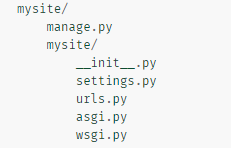
\includegraphics{figuras/3/31/311/img1.png}	 
	 \renewcommand{\arraystretch}{1.3}
	 \caption{Árbol de la carpeta \textbf{mysite}}
  \end{center}
\end{figure}
	\end{minipage}
\end{figure} 
\color{black}{}

Enumeremos estos archivos:

\begin{enumerate}
\item 
El directorio externo \textbf{mysite/root} es un contenedor para su proyecto. Su nombre no le importa a \django{}; puedes cambiarle el nombre a lo que quieras

\item 
\textbf{manage.py:} es una utilidad de línea de comandos que te permite interactuar con este proyecto de \django{} de varias maneras. Puede leer todos los detalles sobre \textit{manage.py} en \textcolor{B}{\href{https://docs.djangoproject.com/en/3.0/ref/django-admin/}{django-admin y manage.py}}.

\item 
El directorio \textbf{mysite/} interno es el paquete real de \py{} para su proyecto. Su nombre es el nombre del paquete \py{} que necesitará usar para importar cualquier cosa dentro de él (\textit{por ejemplo, mysite.urls}). 

\item
\textbf{mysite/\_\_ init\_\_.py:} un archivo vacío que le dice a Python que este directorio debe considerarse un paquete de Python. Si eres un principiante de \py{}, 
{\textcolor{B}{\href{https://docs.python.org/3/tutorial/modules.html}{lee mas sobre estos paquetes en la documentacion oficial  \py{}}}}

\item 
\textbf{mysite/settings.py:}  configuración para este proyecto de \django{}. La configuración de \django{} le dirá todo sobre cómo funciona la configuración ({\textcolor{B}{\href{https://docs.djangoproject.com/en/3.0/topics/settings/}{django settings}}}).

\item 
\textbf{mysite/urls.py:} las declaraciones de URL para este proyecto de \django{}; una "tabla de contenido" de su sitio impulsado por Django. Puede leer más sobre las URL en el
{\textcolor{B}{\href{https://docs.djangoproject.com/en/3.0/topics/http/urls/}{despachador de URL}}}.

\item 
\textbf{mysite/asgi.py:} Un punto de entrada para servidores web compatibles con ASGI para servir su proyecto. Consulte 
{\textcolor{B}{\href{https://docs.djangoproject.com/en/3.0/howto/deployment/asgi/}{Cómo implementar con ASGI}}} para obtener más detalles.

\item 
\textbf{mysite/wsgi.py:} 
Un punto de entrada para servidores web compatibles con WSGI para servir su proyecto. 
 Consulte {\textcolor{B}{\href{https://docs.djangoproject.com/en/3.0/howto/deployment/wsgi/}{Cómo implementar con WSGI}}} para obtener más detalles.

\end{enumerate}

\subsubsection{El servidor de desarrollo}

Verifiquemos que su proyecto \django{} funciona. Cambie al directorio externo de \textbf{mysite}, si aún no lo ha hecho, y ejecute el siguiente comando:
$$
\fbox{\$ python manage.py runserver}
$$
Luego, deberías ver sobre la linea de comandos, algo similar a lo que aparece en la siguiente imagen:

\begin{figure}[H]
  \begin{center}
  	 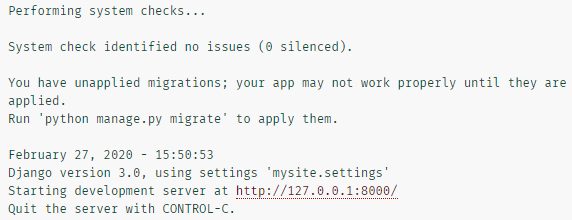
\includegraphics{figuras/3/31/312/img1.png}	 
	 \renewcommand{\arraystretch}{1.3}
	 \caption{Inicio del servidor de django sobre la linea de comandos}
  \end{center}
\end{figure}

Has iniciado el servidor de desarrollo \django{}, un servidor web ligero escrito exclusivamente en \py{}. Hemos incluido esto con \django{} para que pueda desarrollar las cosas rápidamente, sin tener que lidiar con la configuración de un servidor de producción, como \textbf{Apache}, hasta que esté listo para la producción.


Ahora es un buen momento para tener en cuenta que no debe usar este servidor en nada parecido a un entorno de producción. Está destinado solo para su uso durante el desarrollo. 

Ahora que el servidor se está ejecutando, visite $http://127.0.0.1:8000/$ con su navegador web. Verás un \textbf{"¡Felicitaciones!"} sobre la página y con un cohete despegando. Si es asi entonces ¡Funcionó!.

\begin{table}[H]
	%\renewcommand{\arraystretch}{1.3}	
	\begin{tabular}{||c||}
	\hline \\
	\begin{Large}
	\textbf{\textit{Cambiando el puerto}}
	\end{Large}
	\\\\
			De manera predeterminada, el comando runserver inicia el servidor de desarrollo en la IP interna en el puerto 8000.\\
Si desea cambiar el puerto del servidor, páselo como un argumento de línea de comandos.\\Por ejemplo, este comando inicia el servidor en el puerto 8080:
\\\\
$$\fbox{\$ python manage.py runserver 8080}$$
\\\\
Si desea cambiar la IP del servidor, páselo junto con el puerto.\\ Por ejemplo, para escuchar todas las IP públicas disponibles\\ (lo cual es útil si está ejecutando Vagrant o desea mostrar su trabajo en otras computadoras en la red), use:
\\\\$$\fbox{\$ python manage.py runserver 0:8000}$$
\\\\

0 es un atajo para 0.0.0.0. Los documentos completos para el servidor de desarrollo se pueden encontrar en \\la referencia del servidor de ejecución.
	\\ \hline 	
			\end{tabular}
		\end{table}		
		
\begin{table}[H]
	%\renewcommand{\arraystretch}{1.3}	
	\begin{tabular}{||c||}
	\hline \\
	\begin{Large}
	\textbf{\textit{Reinicio automático del servidor}}
	\end{Large}
	\\\\		
El servidor de desarrollo vuelve a cargar automáticamente el código \py{} para cada solicitud según sea necesario.\\ No necesita reiniciar el servidor para que los cambios de código surtan efecto.\\ Sin embargo, algunas acciones como agregar archivos no activan un reinicio, por lo que deberá reiniciar el servidor \\en estos casos.
\\ \hline 	
			\end{tabular}
		\end{table}		

\subsubsection{Creando la aplicación de encuestas (polls)}
Una vez que su entorno de proyecto esta listo y configurado, estamos listos para empezar a trabajar.


Cada aplicación que escribe en \django{} consiste en un paquete de \py{} que sigue una determinada convención. \django{} viene con una utilidad que genera automáticamente la estructura básica de directorios de una aplicación, por lo que puede centrarse en escribir código en lugar de crear directorios.

\begin{table}[H]
	%\renewcommand{\arraystretch}{1.3}	
	\begin{tabular}{||c||}
	\hline \\
	\begin{Large}
	\textbf{\textit{Proyectos Vs Aplicaciones}}
	\end{Large}
	\\\\		
¿Cuál es la diferencia entre un proyecto y una aplicación?\\ Una aplicación es una aplicación web que hace algo, por ejemplo, un sistema de registro web, una base de datos de\\ registros públicos o una pequeña aplicación de encuestas.\\ Un proyecto es una colección de configuraciones y aplicaciones para un sitio web en particular. \\Un proyecto puede contener múltiples aplicaciones.\\ Una aplicación puede estar en múltiples proyectos.
\\ \hline 	
			\end{tabular}
		\end{table}		

Sus aplicaciones pueden vivir en cualquier lugar de su
{\textcolor{B}{\href{https://docs.python.org/3/tutorial/modules.htm}{ruta de Python}}}. En este tutorial, crearemos nuestra aplicación de encuestas justo al lado de su archivo \textit{manage.py} para que pueda importarse como su propio módulo de nivel superior, en lugar de un submódulo de \textit{mysite}.

Para crear su aplicación, asegúrese de estar en el mismo directorio que \textit{manage.py} y escriba este comando:

$$\fbox{\$ python manage.py startapp polls}$$

Eso creará un directorio de encuestas, que se presenta así:

\begin{figure}[H]
  \begin{center}
  	 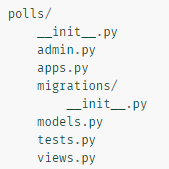
\includegraphics{figuras/3/31/313/img1.png}	 
	 \renewcommand{\arraystretch}{1.3}
	 \caption{directorio de encuestas}
  \end{center}
\end{figure}


Esta estructura de directorios albergará la aplicación de la encuesta.

\subsubsection{Escribiendo la primer vista (view)}

Escribamos la primera vista. Abra el archivo \textbf{polls/views.py} y coloque el siguiente código de \py{}:

\begin{figure}[H]
  \begin{center}
  	 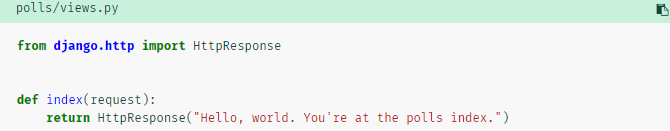
\includegraphics{figuras/3/31/314/img1.png}	 
	 \renewcommand{\arraystretch}{1.3}
	 \caption{Código \py{} de la primer vista}
  \end{center}
\end{figure}


Esta es la vista más simple posible en \django{}. Para llamar a la vista, necesitamos asignarla a una \textbf{URL}, y para esto necesitamos una \textbf{URLconf}.

Para crear una \textbf{URLconf} en el directorio de encuestas, cree un archivo llamado \textit{urls.py}. Su directorio de aplicaciones ahora debería verse como en la \textit{figura 5}
Donde en el archivo \textit{urls.py} ubicado en \textit{polls} se incluirá el código quedando este como el código de la \textit{figura 5}.

\begin{figure}[H]
  \begin{center}
  	 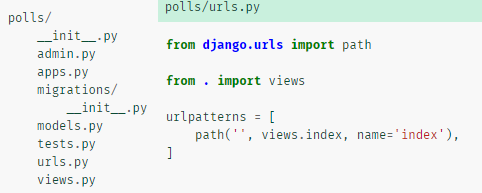
\includegraphics{figuras/3/31/314/img2.png}	 
	 \renewcommand{\arraystretch}{1.3}
	 \caption{Modificacion del directorio polls y agregado del codigo sobre el \textit{urls.py}}
  \end{center}
\end{figure}

El siguiente paso es apuntar la \textbf{URLconf} raíz al módulo \textit{polls.urls}. En \textbf{mysite/urls.py}, agregue una importación para \textcolor{G}{django.urls.include} e inserte un \textcolor{B}{\textit{include}}() en la lista \textit{urlpatterns}, Debe quedar como en la \textit{figura 6}.

\begin{figure}[H]
  \begin{center}
  	 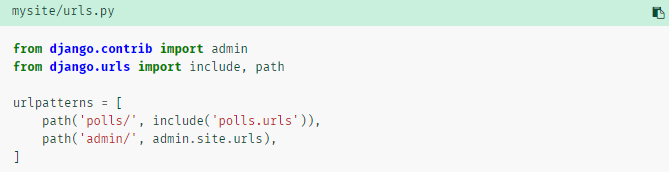
\includegraphics{figuras/3/31/314/img3.png}	 
	 \renewcommand{\arraystretch}{1.3}
	 \caption{Modificacion del codigo sobre el \textit{urls.py} del proyecto}
  \end{center}
\end{figure}

La función {\href{https://docs.djangoproject.com/en/3.0/ref/urls/#django.urls.include}{\textcolor{B}{\textit{include}}()}} permite hacer referencia a otros \textbf{URLconfs}. Cada vez que \django{} se encuentra con {\href{https://docs.djangoproject.com/en/3.0/ref/urls/#django.urls.include}{\textcolor{B}{\textit{include}}()}}, corta cualquier parte de la \textbf{URL} que coincida con ese punto y envía la cadena restante a la \textbf{URLconf} incluida para su posterior procesamiento.


La idea detrás de {\href{https://docs.djangoproject.com/en/3.0/ref/urls/#django.urls.include}{\textcolor{B}{\textit{include}}()}} es facilitar la conexión y reproducción de \textbf{URL}. Como las encuestas están en su propia \textbf{URLconf} (\textbf{polls/urls.py}), se pueden colocar debajo de \textit{/polls/}, o debajo de \textit{/fun\_ polls/}, o debajo de \textit{/content/polls/}, o cualquier otra ruta raíz, y la aplicación seguirá funcionando.

\begin{table}[H]
	%\renewcommand{\arraystretch}{1.3}	
	\begin{tabular}{||c||}
	\hline \\
	\begin{Large}
	\textbf{\textit{Cuando usamos include()}}
	\end{Large}
	\\\\		
Siempre debe usar {\href{https://docs.djangoproject.com/en/3.0/ref/urls/#django.urls.include}{\textcolor{B}{\textit{include}}()}} cuando incluya otros patrones de \textbf{URL}. \textcolor{G}{admin.site.urls} es la única excepción a esto.
\\ \hline 	
			\end{tabular}
		\end{table}		


Ahora ha conectado una vista de índice en la \textbf{URLconf}. Verifique que esté funcionando con el siguiente comando:
$$\fbox{\$ python manage.py runserver}$$


Vaya a \textit{http://localhost:8000/polls/} en su navegador, y debería ver el texto \textit{"Hello, world. You're at the polls index"}, que definiste en la vista de índice.

\begin{table}[H]
	%\renewcommand{\arraystretch}{1.3}	
	\begin{tabular}{||c||}
	\hline \\
	\begin{Large}
	\textbf{\textit{Te aparece \textbf{Page Not Found?}}}
	\end{Large}
	\\\\		
Si recibe una página de error aquí, verifique que vaya a \textit{http://localhost:8000/polls/} y no \textit{http://localhost:8000/}.
\\\\ \hline 	
			\end{tabular}
		\end{table}		

La función {\href{https://docs.djangoproject.com/en/3.0/ref/urls/#django.urls.path
}{\textcolor{B}{\textit{path}}()}} recibe cuatro argumentos, dos obligatorios: ruta y vista, y dos opcionales: kwargs y nombre. En este punto, vale la pena revisar para qué sirven estos argumentos.

\begin{itemize}
\item \textbf{\textit{Argumento route del path():}}

\textit{route} es una cadena que contiene un patrón de \textbf{URL}. Al procesar una solicitud, \django{} comienza en el primer patrón en \textit{urlpatterns} y avanza por la lista, comparando la \textbf{URL} solicitada con cada patrón hasta que encuentre uno que coincida.

Los patrones no buscan parámetros \textbf{GET} y \textbf{POST}, o el nombre de dominio. \textit{Por ejemplo}, en una solicitud a \textit{https://www.example.com/myapp/}, la \textbf{URLconf} buscará \textbf{myapp/}. En una solicitud a 

\textit{https://www.example.com/myapp/?page=3}, la \textbf{URLconf} también buscará \textbf{myapp/}.

\item \textbf{\textit{Argumento view del path():}}

Cuando \django{} encuentra un patrón coincidente, llama a la función de vista especificada con un objeto {\textcolor{B}{\href{https://docs.djangoproject.com/en/3.0/ref/request-response/}{HttpRequest}}} como primer argumento y cualquier valor ``capturado" de la ruta como argumentos de palabras clave. Vamos a dar un ejemplo de esto en un momento.

\item \textbf{\textit{Argumento kwargs del path():}}

Los argumentos de palabras clave arbitrarias se pueden pasar en un diccionario a la vista de destino. No vamos a utilizar esta función de Django en el tutorial.

\item \textbf{\textit{Argumento name del path():}}


Nombrar su \textbf{URL} le permite referirse a ella sin ambigüedades desde otros lugares de \django{}, especialmente desde las plantillas. Esta poderosa característica le permite realizar cambios globales en los patrones de \textbf{URL} de su proyecto mientras solo toca un solo archivo.
\end{itemize}

\subsection{Escribiendo tu primera aplicación \django{}, parte 2}
\subsubsection{Configuración de la Base de Datos}
Ahora, abra \textbf{mysite/settings.py}. Es un módulo \py{} normal con variables de nivel de módulo que representan la configuración de \django{}.

Por defecto, la configuración usa \textbf{SQLite}. Si eres nuevo en las bases de datos, o simplemente estás interesado en probar \django{}, esta es la opción más fácil. \textbf{SQLite} está incluido en \py{}, por lo que no necesitará instalar nada más para admitir su base de datos. Sin embargo, al comenzar su primer proyecto real, es posible que desee utilizar una base de datos más escalable como \textbf{PostgreSQL}, para evitar dolores de cabeza de cambio de base de datos en el futuro.

Si desea utilizar otra base de datos, instale los enlaces de base de datos apropiados {\textcolor{B}{\href{https://docs.djangoproject.com/en/3.0/topics/install/\#database-installation}{(database bindings)}}}
 y cambie las siguientes claves en el elemento {\textcolor{B}{\href{https://docs.djangoproject.com/en/3.0/ref/settings/\#std:setting-DATABASES}{DATABASES}}} 'default' para que coincida con la configuración de conexión de su base de datos:

\begin{itemize}
\item \textcolor {B}{\href{https://docs.djangoproject.com/en/3.0/ref/settings/\#std:setting-DATABASE-ENGINE}{ENGINE}} - Puede ser: \textcolor{G}{'django.db.backends.sqlite3'}, \textcolor{G}{'django.db.backends.postgresql'}, \textcolor{G}{'django.db.backends.mysql'}, or \textcolor{G}{'django.db.backends.oracle'}. 
Otros backends también están 
\textcolor {B}{\href{https://docs.djangoproject.com/en/3.0/ref/databases/\#third-party-notes}{disponibles}}.

\item \textcolor {B}{\href{https://docs.djangoproject.com/en/3.0/ref/settings/\#std:setting-NAME}{NAME}} - 
El nombre de su base de datos. Si está utilizando \textbf{SQLite}, la base de datos será un archivo en su computadora; en ese caso, \textcolor {B}{\href{https://docs.djangoproject.com/en/3.0/ref/settings/\#std:setting-NAME}{NAME}} debe ser la ruta absoluta completa, incluido el nombre de archivo, de ese archivo. El valor predeterminado, \textcolor{G}{os.path.join (BASE\_DIR, 'db.sqlite3')}, almacenará el archivo en el directorio de su proyecto.

\end{itemize}

Si no está utilizando \textbf{SQLite} como su base de datos, se deben agregar configuraciones adicionales como \textcolor {B}{\href{https://docs.djangoproject.com/en/3.0/ref/settings/\#std:setting-USER}{USUARIO}}
, \textcolor {B}{\href{https://docs.djangoproject.com/en/3.0/ref/settings/\#std:setting-PASSWORD}{CONTRASEÑA}}
 y \textcolor {B}{\href{https://docs.djangoproject.com/en/3.0/ref/settings/\#std:setting-HOST}{HOST}}
. Para obtener más detalles, consulte la documentación de referencia para \textcolor {B}{\href{https://docs.djangoproject.com/en/3.0/ref/settings/\#std:setting-DATABASES}{BASES DE DATOS}}.

\begin{table}[H]
	%\renewcommand{\arraystretch}{1.3}	
	\begin{tabular}{||c||}
	\hline \\
	\begin{Large}
	\textbf{\textit{Para bases de datos que no sean SQLite}}
	\end{Large}
	\\\\		
Si está utilizando una base de datos además de \textbf{SQLite}, asegúrese de haber creado una base de datos\\ en este momento. Haga eso con \textcolor{G}{$"CREATE$ $DATABASE$ $database\_name;"$} dentro de la solicitud \\interactiva de su base de datos.
También asegúrese de que el usuario de la base de datos proporcionado en\\ \textbf{mysite/settings.py} tenga privilegios de "crear base de datos". Esto permite la creación automática\\ de una base de datos de prueba que será necesaria en un tutorial posterior.\\
Si está utilizando \textbf{SQLite}, no necesita crear nada de antemano; el archivo de la base de datos se creará\\ automáticamente cuando sea necesario.
\\\\ \hline 	
			\end{tabular}
		\end{table}		


Mientras editas \textbf{mysite/settings.py}, configura {\textcolor{B}{\href{https://docs.djangoproject.com/en/3.0/ref/settings/\#std:setting-TIME\_ZONE}{TIME\_ZONE}}}
 en su zona horaria.

Además, tenga en cuenta la configuración {\textcolor{B}{\href{https://docs.djangoproject.com/en/3.0/ref/settings/\#std:setting-INSTALLED\_APPS}{INSTALLED\_APPS}}}
 en la parte superior del archivo. Esta contiene los nombres de todas las aplicaciones de \django{} que se activan en esta instancia de \django{}. Las aplicaciones se pueden usar en múltiples proyectos, y puede empaquetarlas y distribuirlas para que otras personas las usen en sus proyectos.


Por defecto, {\href{https://docs.djangoproject.com/en/3.0/ref/settings/\#std:setting-INSTALLED\_APPS}{INSTALLED\_APPS}} contiene las siguientes aplicaciones, las cuales se instalan al instalar \django{} 

\begin{itemize}
%{\href{}{\textcolor{B}{}}}
%1
\item {\href{https://docs.djangoproject.com/en/3.0/ref/contrib/admin/\#module-django.contrib.admin}{\textcolor{B}{django.contrib.admin}}} – Sitio de administración.
%2
\item {\href{https://docs.djangoproject.com/en/3.0/topics/auth/\#module-django.contrib.auth}{\textcolor{B}{django.contrib.auth}}} – Sistema de autenticación.
%3
\item {\href{https://docs.djangoproject.com/en/3.0/ref/contrib/contenttypes/\#module-django.contrib.contenttypes}{\textcolor{B}{django.contrib.contenttypes}}} – 
Un marco para los tipos de contenido.
%4
\item {\href{https://docs.djangoproject.com/en/3.0/topics/http/sessions/\#module-django.contrib.sessions}{\textcolor{B}{django.contrib.sessions}}} – framework (marco) de sesiones.
%5
\item {\href{https://docs.djangoproject.com/en/3.0/ref/contrib/messages/\#module-django.contrib.messages}{\textcolor{B}{django.contrib.messages}}} – framework (marco) de mensajes.
%6
\item {\href{https://docs.djangoproject.com/en/3.0/ref/contrib/staticfiles/\#module-django.contrib.staticfiles}{\textcolor	{B}{django.contrib.staticfiles}}} – 
Un marco para administrar archivos estáticos.

\end{itemize}

Estas aplicaciones se incluyen por defecto como una conveniencia para casos específicos.

Sin embargo, algunas de estas aplicaciones utilizan al menos una tabla de base de datos, por lo que debemos crear las tablas en la base de datos antes de poder usarlas. Para hacer eso, ejecuta el siguiente comando:

$$\fbox{\$ python manage.py migrate}$$

El comando migrate analiza la configuración {\href{https://docs.djangoproject.com/en/3.0/ref/settings/\#std:setting-INSTALLED\_APPS}{\textcolor{B}{INSTALLED\_APPS}}} y crea las tablas de base de datos necesarias de acuerdo con la configuración de la base de datos en su archivo \textbf{mysite/settings.py} y las migraciones de la base de datos que se envían con la aplicación (las cubriremos más adelante). Verá un mensaje para cada migración que aplique. Si está interesado, ejecute el cliente de línea de comandos para su base de datos y escriba \textbackslash dt (PostgreSQL), MOSTRAR TABLAS; (MariaDB, MySQL), .schema (SQLite) o SELECT TABLE\_NAME FROM USER\_TABLES; (Oracle) para mostrar las tablas que Django creó.

\begin{table}[H]
	%\renewcommand{\arraystretch}{1.3}	
	\begin{tabular}{||c||}
	\hline \\
	\begin{Large}
	\textbf{\textit{Para los minimalistas}}
	\end{Large}
	\\\\		
Como dijimos anteriormente, las aplicaciones predeterminadas se incluyen para el caso común, pero no todos\\ las necesitan. Si no necesita ninguno o todos ellos, no dude en comentar o eliminar las líneas apropiadas de\\ {\href{https://docs.djangoproject.com/en/3.0/ref/settings/\#std:setting-INSTALLED\_APPS}{\textcolor{B}{INSTALLED\_APPS}}} antes de ejecutar la {\href{https://docs.djangoproject.com/en/3.0/ref/django-admin/\#django-admin-migrate}{\textcolor{B}{migración}}}
.\\ El comando {\href{https://docs.djangoproject.com/en/3.0/ref/django-admin/\#django-admin-migrate}{\textcolor{B}{migrate}}}
 solo ejecutará migraciones para aplicaciones en {\href{https://docs.djangoproject.com/en/3.0/ref/settings/\#std:setting-INSTALLED\_APPS}{\textcolor{B}{INSTALLED\_APPS}}}.
\\\\ \hline 	
			\end{tabular}
		\end{table}		

\subsubsection{Creando un Modelo}

\begin{table}[H]
	%\renewcommand{\arraystretch}{1.3}	
	\begin{tabular}{||c||}
	\hline \\
	\begin{Large}
	\textbf{\textit{Filosofia}}
	\end{Large}
	\\\\		
Un modelo es la fuente única y definitiva de verdad sobre sus datos. Contiene los campos y \\comportamientos esenciales de los datos que está almacenando.\\ \django{} sigue el principio DRY ({\href{https://docs.djangoproject.com/en/3.0/misc/design-philosophies/\#dry}{\textcolor{B}{DRY principle}}}).\\ El objetivo es definir su modelo de datos en un lugar y derivar automáticamente cosas de él.\\

Esto incluye las migraciones, a diferencia de \textbf{Ruby On Rails}, por ejemplo, las migraciones\\ se derivan completamente de su archivo de modelos, y son esencialmente un historial que\\ \django{} puede recorrer para actualizar su esquema de base de datos para que coincida con sus\\ modelos actuales.
\\\\ \hline 	
			\end{tabular}
		\end{table}		

En nuestra aplicación de encuestas, crearemos dos modelos: Pregunta (Question) y Elección (Choice). 

\begin{figure}[H]
	\begin{center}
		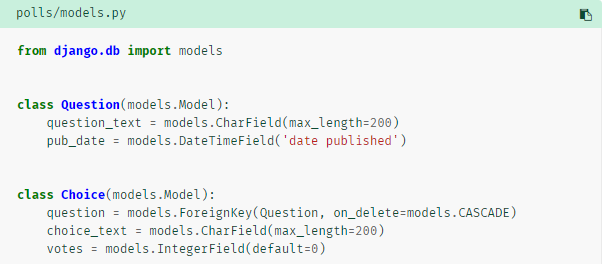
\includegraphics[scale=0.7]{figuras/3/32/322/img1.png}
		\renewcommand{\arraystretch}{1.3}
		\caption{Codigo de los modelos \textbf{Question} y \textbf{Choice}}
	\end{center}
\end{figure}
Una Question tiene una pregunta y una fecha de publicación. Una opción tiene dos campos: el texto de la opción y un conteo de votos. Cada opción está asociada con una pregunta.

Estos conceptos están representados por las clases de \py. Edite el archivo \textbf{polls/models.py} para que se vea como en la \textit{figura 7}.

Aquí, cada modelo está representado por una clase que subclasifica {\href{https://docs.djangoproject.com/en/3.0/ref/models/instances/\#django.db.models.Model}{\textcolor{B}{django.db.models.Model}}}	. Cada modelo tiene una serie de variables de clase, cada una de las cuales representa un campo de base de datos en el modelo.

Cada campo está representado por una instancia de clase {\href{https://docs.djangoproject.com/en/3.0/ref/models/fields/\#django.db.models.Field}{\textcolor{B}{Campo}}}, por ejemplo, {\href{https://docs.djangoproject.com/en/3.0/ref/models/fields/\#django.db.models.CharField}{\textcolor{B}{CharField}}} para campos de caracteres y {\href{https://docs.djangoproject.com/en/3.0/ref/models/fields/\#django.db.models.DateTimeField}{\textcolor{B}{DateTimeField}}}
 para fechas y horas. Esto le dice a \django{} qué tipo de datos contiene cada campo.

El nombre de cada instancia de campo (por ejemplo, question\_text o pub\_date) es el nombre del campo, en formato amigable para la máquina. Utilizará este valor en su código de \py{}, y su base de datos lo usará como el nombre de la columna

Puede usar un primer argumento posicional opcional del campo para designar un nombre que sea legible por humanos. Eso se usa en un par de partes introspectivas de \django{}, y también sirve como documentación. Si no se proporciona este campo, \django{} usará el nombre legible por la máquina. En este ejemplo, solo hemos definido un nombre legible para humanos para \textcolor{G}{Question.pub\_date}. Para todos los demás campos en este modelo, el nombre del campo legible por la máquina será suficiente como su nombre legible por humanos.

Algunas clases de campo tienen argumentos requeridos. {\href{https://docs.djangoproject.com/en/3.0/ref/models/fields/\#django.db.models.CharField}{\textcolor{B}{CharField}}}, por ejemplo, requiere que le des una \textbf{longitud máxima} ({\href{https://docs.djangoproject.com/en/3.0/ref/models/fields/\#django.db.models.CharField.max_length}{\textcolor{B}{max\_length}}}). Eso se usa no solo en el esquema de la base de datos, sino también en la validación.

Un campo también puede tener varios argumentos opcionales; en este caso, hemos establecido el valor predeterminado ({\href{https://docs.djangoproject.com/en/3.0/ref/models/fields/\#django.db.models.Field.default}{\textcolor{B}{default}}}) de votos en 0.

Finalmente, tenga en cuenta que se define una relación, usando {\href{https://docs.djangoproject.com/en/3.0/ref/models/fields/#django.db.models.ForeignKey}{\textcolor{B}{ForeingKey}}}
. Eso le dice a \django{} que cada Elección está relacionada con una sola Pregunta. \django{} admite todas las relaciones de base de datos comunes: muchas a una, muchas a muchas y una a una.


\subsubsection{Modelos de Activación}

Ese pequeño fragmento de código del modelo le da a \django{} bastante información. Con él, \django{} es capaz de:
\begin{itemize}
\item 
Crear un esquema de base de datos (sentencias CREATE TABLE) para esta aplicación.
\item
Crear una \textbf{API} de acceso a la base de datos de \py{} para acceder a los objetos \textbf{Question} y \textbf{Choice}.
\end{itemize}

Pero primero debemos decirle a nuestro proyecto \textit{que la aplicación de encuestas está instalada}.


\begin{table}[H]
	%\renewcommand{\arraystretch}{1.3}	
	\begin{tabular}{||c||}
	\hline \\
	\begin{Large}
	\textbf{\textit{Filosofia}}
	\end{Large}
	\\\\		
Las aplicaciones de \django{} son "conectables": puede usar una aplicación en varios proyectos y puede\\ distribuir aplicaciones,ya que no tienen que estar vinculadas a una determinada instalación de \django{}.
\\\\ \hline 	
			\end{tabular}
		\end{table}		


Para incluir la aplicación en nuestro proyecto, necesitamos agregar una referencia a su clase de configuración en la configuración {\href{https://docs.djangoproject.com/en/3.0/ref/settings/\#std:setting-INSTALLED\_APPS}{\textcolor{B}{INSTALLED\_APPS}}}. La clase \textcolor{G}{PollsConfig} está en el archivo \textbf{polls/apps.py}, por lo que su ruta punteada es \textcolor{G}{'polls.apps.PollsConfig'}. Hay que editar el archivo mysite/settings.py y agreguar esa ruta punteada a la configuración {\href{https://docs.djangoproject.com/en/3.0/ref/settings/\#std:setting-INSTALLED\_APPS}{\textcolor{B}{INSTALLED\_APPS}}}. Se verá así:

\begin{figure}[H]
	\begin{center}
		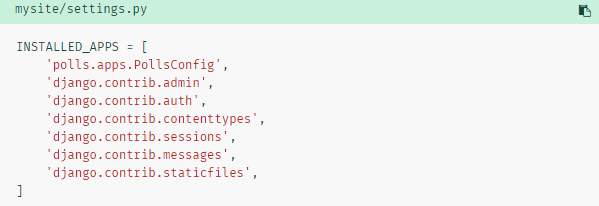
\includegraphics[scale=0.9]{figuras/3/32/323/img1.png}
		\renewcommand{\arraystretch}{1.3}
		\caption{Instalación de la aplicación polls en el \textcolor{G}{settings.py} del proyecto }
	\end{center}
\end{figure}


Listo, \django{} con esto ya sabe incluir la aplicación de encuestas. Ahora, debemos aplicar migraciones, lo cual se hace con el comando:

$$\fbox{\$ python manage.py makemigrations polls}$$

Luego, en la terminal vas a ver algo similar a:

\begin{figure}[H]
\begin{center}
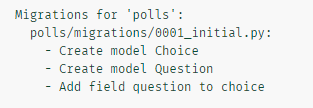
\includegraphics[scale=1]{figuras/3/32/323/img2.png}
\renewcommand{\arraystretch}{1.3}
\caption{Terminal con un makemigrations satisfactorio}
\end{center}
\end{figure}


Al correr \textit{makemigrations}, le estás diciendo a Django que has realizado algunos cambios en tus modelos (En este caso, agregaste modelos al \textbf{models.py}) y que queremos que esos cambios sean almacenados como migraciones.


Las migraciones es la forma en la cual \django{} almacena los cambios en sus modelos (y, por lo tanto, en el esquema de su base de datos): estos son archivos en el disco. Podemos leer las migraciones si queremos; en este caso son las encuestas de \textbf{polls/migrations/0001\_initial.py}. No se preocupe, no se espera que los lea cada vez que Django hace uno, pero están diseñados para ser editados por humanos en caso de que desee modificar manualmente cómo \django{} cambia las cosas.


Hay un comando que ejecutará las migraciones por usted y administrará el esquema de su base de datos automáticamente, este es el comando \textit{migrate}, y lo veremos en un momento, pero primero, veamos qué \textbf{SQL} ejecutará esa migración. El comando \textit{sqlmigrate} toma nombres de migración y devuelve su SQL:

$$\fbox{\$ python manage.py sqlmigrate polls 0001}$$

Vas a ver algo similar a esto, quizas en otro formato pero con el mismo contenido:


\begin{figure}[H]
\begin{center}
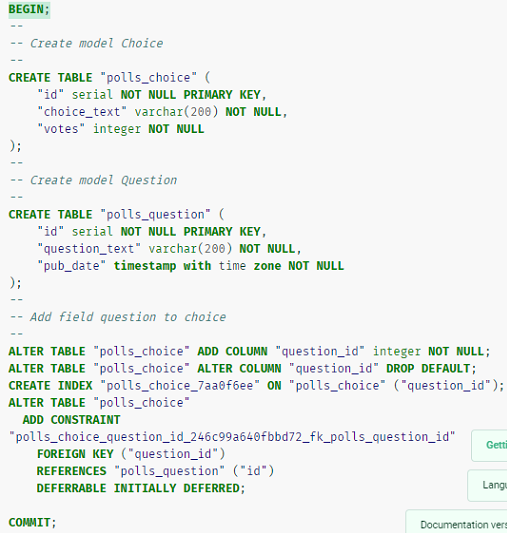
\includegraphics[scale=0.7]{figuras/3/32/323/img3.png}
\renewcommand{\arraystretch}{1.3}
\caption{python manage.py sqlmigrate polls 0001}
\end{center}
\end{figure}

Notemos que:

\begin{itemize}
\item 
El resultado exacto variará según la base de datos que esté utilizando. El ejemplo anterior se genera para PostgreSQL.

\item
Los nombres de las tablas se generan automáticamente combinando el nombre de la aplicación (encuestas) y el nombre en minúsculas del modelo: pregunta y elección. (Puede anular este comportamiento).

\item 
Las claves primarias (ID) se agregan automáticamente. (También puede anular esto).

\item 
Por convención, \django{} agrega "\_id" al nombre del campo de clave externa. (Sí, también puedes sobrescribirlo).

\item 
La relación de clave externa se hace explícita por una restricción FOREIGN KEY. No se preocupe por las partes DEFERRABLES; esto le dice a PostgreSQL que no aplique la clave foránea hasta el final de la transacción

\item 
Se adapta a la base de datos que está utilizando, por lo que los tipos de campo específicos de la base de datos como auto\_increment (MySQL), serial (PostgreSQL) o autoincrement de clave primaria entera (SQLite) se manejan automáticamente. Lo mismo ocurre con las citas de los nombres de campo, por ejemplo, con comillas dobles o comillas simples.

\item 
El comando \textit{sqlmigrate} no ejecuta realmente la migración en su base de datos, sino que lo imprime en la pantalla para que pueda ver lo que \textbf{SQL Django} cree que es necesario. Es útil para verificar qué hará \django{} o si tiene administradores de bases de datos que requieren \textit{scripts SQL} para dichos cambios.
\end{itemize}

Si está interesado, también puede ejecutar \textit{python manage.py check}; Esto verifica si hay algún problema en su proyecto sin hacer migraciones o tocar la base de datos.

Ahora, debemos correr el comando \textit{migrate} otra vez para crear estos modelos en las tablas de tu base de datos.

\begin{figure}[H]
\begin{center}
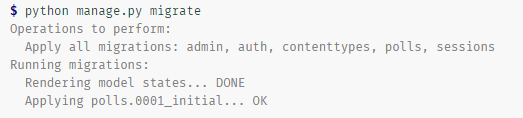
\includegraphics[scale=1]{figuras/3/32/323/img4.png}
\renewcommand{\arraystretch}{1.3}
\caption{python manage.py sqlmigrate polls 0001}
\end{center}
\end{figure}


El comando \textit{migrate} toma todas las migraciones que no se han aplicado (\django{} rastrea cuáles se aplican usando una tabla especial en su base de datos llamada \textcolor{G}{django\_migrations}) y las ejecuta en su base de datos, esencialmente, sincronizando los cambios que realizó en sus modelos con el esquema en la base de datos.

Las migraciones son muy potentes y le permiten cambiar sus modelos con el tiempo, a medida que desarrolla su proyecto, sin la necesidad de eliminar su base de datos o tablas y crear nuevas: se especializa en actualizar su base de datos en vivo, sin perder datos. Los cubriremos con más profundidad en una parte posterior del tutorial, pero por ahora, recuerde la guía de tres pasos para realizar cambios en el modelo:

\begin{itemize}
\item
Creamos/modificamos los modelos en el archivo \textit{models.py}.

\item
Luego corremos el comando \textit{python manage.py makemigrations} para crear las migraciones para esos cambios.

\item
Corremos el comando \textit{python manage.py migrate} para aplicar los cambios realizados en la base de datos.
\end{itemize}

La razón por la que existen comandos separados para realizar y aplicar migraciones es porque comprometerás las migraciones en tu sistema de control de versiones y las enviarás con tu aplicación; no solo facilitan su desarrollo, también pueden ser utilizados por otros desarrolladores y en producción.

\subsubsection{Jugando con la API}

Ahora, entremos al \textit{shell} interactivo de \py{} y juguemos con la \textbf{API} gratuita que \django{} le brinda. Para invocar el \textit{shell} de \py{}, use este comando:

$$\fbox{\$ python manage.py shell}$$


Estamos usando esto en lugar de simplemente escribir \textit{"python"}, porque \textit{manage.py} establece la variable de entorno \textcolor{G}{DJANGO\_SETTINGS\_MODULE}, que le da a \django{} la ruta de importación de \py{} a su archivo \textbf{mysite/settings.py}.

Una ves que entramos en la \textit{shell} podemos trabajar con ella realizando {\href{https://docs.djangoproject.com/en/3.0/topics/db/queries/}{\textcolor{B}{consultas}}} como se indica en la figura:
\begin{figure}[H]
\begin{center}
\renewcommand{\arraystretch}{1.3}
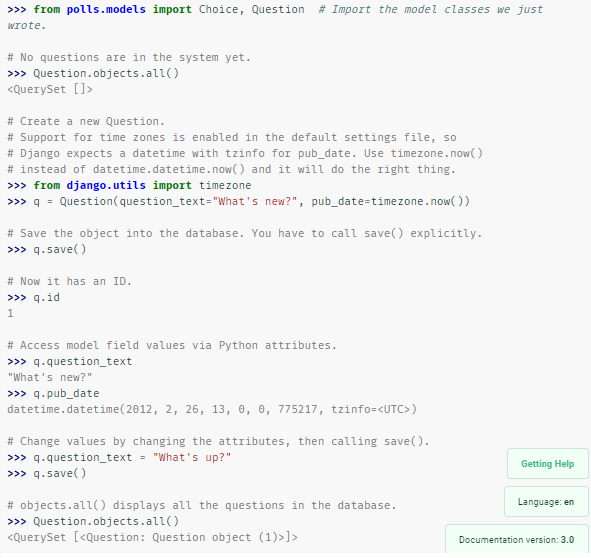
\includegraphics[scale=1.1]{figuras/3/32/324/img1.png}
\caption{Making queries}
\end{center}
\end{figure}


Ahora, vemos una cosa \textbf{$<$Question: Question object (1)$>$} no es una representación útil de este objeto. Arreglemos eso editando el modelo Question (en el archivo \textbf{polls/models.py}) y agregando un método{\href{https://docs.djangoproject.com/en/3.0/ref/models/instances/\#django.db.models.Model.\_\_str\_\_()}{\textcolor{B}{\_\_str \_\_()}}}  a los modelos \textbf{Question} y \textbf{Choice}:
\newpage
\begin{figure}[H]
\begin{center}
\renewcommand{\arraystretch}{1.3}
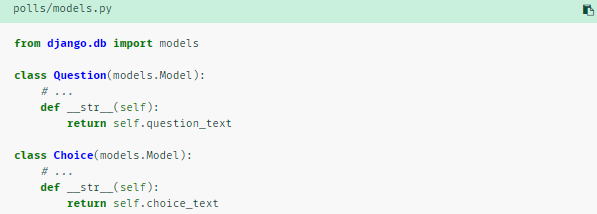
\includegraphics[scale=1]{figuras/3/32/324/img2.png}
\caption{•}
\end{center}
\end{figure}

Es importante agregar los métodos {\href{https://docs.djangoproject.com/en/3.0/ref/models/instances/\#django.db.models.Model.\_\_str\_\_()}{\textcolor{B}{\_\_str \_\_()}}} a sus modelos, no solo para su propia conveniencia al tratar con el mensaje interactivo, sino también porque las representaciones de los objetos se utilizan en todo el administrador generado automáticamente por \django{}.

Agreguemos también un método personalizado a este modelo:
\\
\begin{figure}[H]
\begin{center}
\renewcommand{\arraystretch}{1.3}
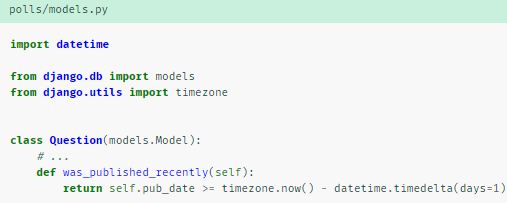
\includegraphics[scale=1]{figuras/3/32/324/img3.png}
\caption{•}
\end{center}
\end{figure}

Observe la adición de \textcolor{G}{import datetime} y de \textcolor{G}{django.utils import timezone}, para hacer referencia al módulo de fecha y hora estándar de \py{} y las utilidades relacionadas con la zona horaria de \django{} en \textcolor{G}{django.utils.timezone}, respectivamente. Si no está familiarizado con el manejo de zona horaria en \py{}, puede obtener más información en los documentos de soporte de zona horaria.


Guarde estos cambios e inicie un nuevo \textit{shell} interactivo de \py{} ejecutando nuevamente \textit{python manage.py shell}:

\begin{figure}[H]
\begin{center}
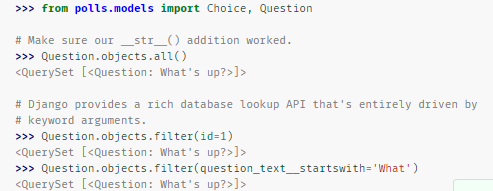
\includegraphics[scale=1]{figuras/3/32/324/img4.png}
\end{center}
\end{figure}
\begin{figure}[H]
\begin{center}
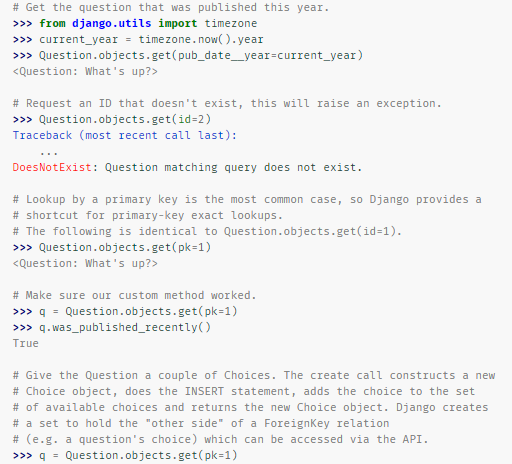
\includegraphics[scale=1]{figuras/3/32/324/img5.png}
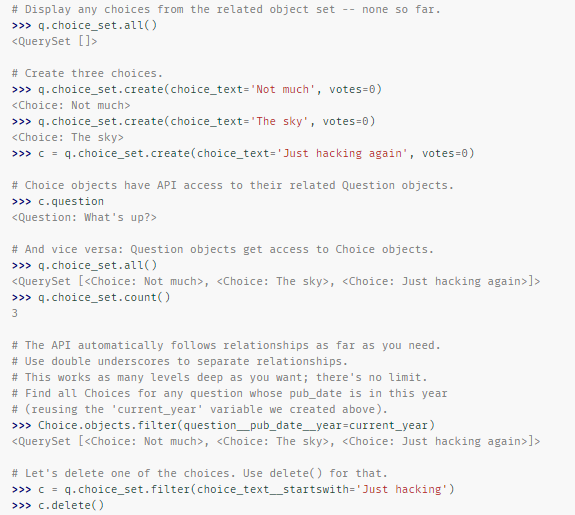
\includegraphics[scale=0.9]{figuras/3/32/324/img6.png}
\end{center}
\end{figure}

Para obtener más información sobre las relaciones del modelo, consulte Acceso a objetos relacionados ({\href{https://docs.djangoproject.com/en/3.0/ref/models/relations/}{\textcolor{B}{Accessing related objects}}}
). Para obtener más información sobre cómo utilizar guiones bajos dobles para realizar búsquedas de campo a través de la API, consulte las búsquedas de campo ({\href{https://docs.djangoproject.com/en/3.0/topics/db/queries/\#field-lookups-intro}{\textcolor{B}{field lookups}}}
). Para obtener detalles completos sobre la API de base de datos, consulte nuestra referencia de API de base de datos ({\href{https://docs.djangoproject.com/en/3.0/topics/db/queries/}{\textcolor{B}{Database API reference}}}).

\subsubsection{Introducción al administrador de \django{}}

\begin{table}[H]
	%\renewcommand{\arraystretch}{1.3}	
	\begin{tabular}{||c||}
	\hline \\
	\begin{Large}
	\textbf{\textit{Filosofia}}
	\end{Large}
	\\\\		
Generar sitios de administración para que su personal o clientes agreguen, cambien y eliminen\\ contenido es un trabajo tedioso que no requiere mucha creatividad. Por esa razón, \django{}\\ automatiza por completo la creación de interfaces de administración para modelos.\\

\django{} fue escrito en un entorno de redacción, con una separación muy clara entre los \\ ``editores de contenido'' y el sitio ``público''.\\ Los administradores del sitio usan el sistema para agregar noticias, \\ eventos, resultados deportivos, etc., y ese contenido se muestra en el sitio público.\\ \django{} resuelve el problema de crear una interfaz unificada para que los administradores \\ del sitio editen contenido.\\

El administrador no está destinado a ser utilizado por los visitantes del sitio.\\ Es para los administradores del sitio.
\\\\ \hline 	
			\end{tabular}
		\end{table}		

\subsubsection*{Creando un usuario administrador}

Crear un usuario administrador Primero, necesitaremos crear un usuario que pueda iniciar sesión en el sitio de administración. Ejecute el siguiente comando:

$$\fbox{\$ python manage.py createsuperuser}$$

Al correr este comando nos pedira una serie de datos, como el nombre del \textit{usuario}, \textit{nuestro mail} y una \textit{contraseña}.

\subsubsection*{Corremos el servidor de desarrollo}
El administrador de \django{} ya viene activado por defecto. 
Primero debemos correr el servidor una vez creado el administrador:

$$\fbox{\$ python manage.py runserver}$$


Ahora, abra un navegador web y vaya a \textbf{/ admin /} en su dominio local, por ejemplo, \textbf{http://127.0.0.1:8000/admin/}. Debería ver la pantalla de inicio de sesión del administrador:

\begin{figure}[H]
\begin{center}
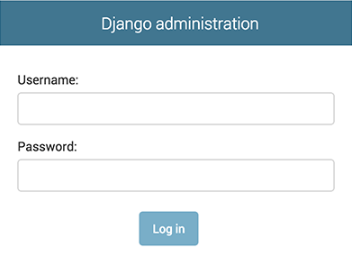
\includegraphics[scale=0.9]{figuras/3/32/325/img1.png}
\caption{Login del administrador}
\end{center}
\end{figure}


Dado que la traducción ({\href{https://docs.djangoproject.com/en/3.0/topics/i18n/translation/}{\textcolor{B}{traslation}}}
) está activada de manera predeterminada, la pantalla de inicio de sesión puede mostrarse en su propio idioma, según la configuración de su navegador y si \django{} tiene una traducción para este idioma.

\subsubsection*{El sitio de administración}

Ahora, intente iniciar sesión con la cuenta de \textit{superusuario} que creó en el paso anterior. Debería ver la página de índice de administración de \django{}:

\begin{figure}[H]
\begin{center}
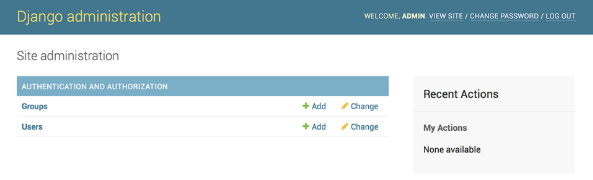
\includegraphics[scale=0.9]{figuras/3/32/325/img2.png}
\caption{Login del administrador}
\end{center}
\end{figure}


Debería ver algunos tipos de contenido editable: grupos y usuarios. Estos los proporciona {\href{https://docs.djangoproject.com/en/3.0/topics/auth/#module-django.contrib.auth}{\textcolor{B}{django.contrib.auth}}}
, el cual es el \textit{marco de autenticación} enviado por \django{}.

\subsubsection*{Hacer que la aplicación de la aplicacion sea modificable en el administrador}

¿Pero dónde está nuestra aplicación de encuestas? No se muestra en la página de índice de administrador.

Solo una cosa más que hacer: necesitamos decirle al administrador que los objetos de Pregunta tienen una interfaz de administrador. Para hacer esto, abra el archivo \textbf{polls/admin.py} y edítelo para que se vea así:

\begin{figure}[H]
\begin{center}
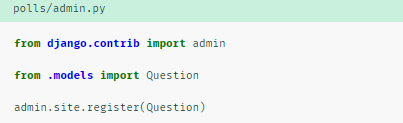
\includegraphics[scale=0.9]{figuras/3/32/325/img3.png}
\caption{Login del administrador}
\end{center}
\end{figure}

\subsubsection*{Explore la funcionalidad de administración gratuita}


Ahora que hemos registrado el modelo \textbf{Question}, \django{} sabe que debería mostrarse en la página de índice de administración:

\begin{figure}[H]
\begin{center}
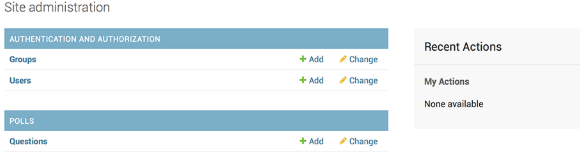
\includegraphics[scale=0.9]{figuras/3/32/325/img4.png}
\caption{Login del administrador}
\end{center}
\end{figure}


Haga clic en \textbf{``Question''}. Ahora está en la página de "lista de cambios" para Question. Esta página muestra todas las preguntas en la base de datos y le permite elegir una para cambiarla. Ahí está el "¿Qué pasa?" pregunta que creamos anteriormente:

\begin{figure}[H]
\begin{center}
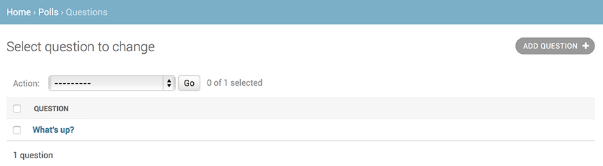
\includegraphics[scale=0.9]{figuras/3/32/325/img5.png}
\caption{Login del administrador}
\end{center}
\end{figure}


Haz clic en "¿Qué pasa?" pregunta para editarlo:

\begin{figure}[H]
\begin{center}
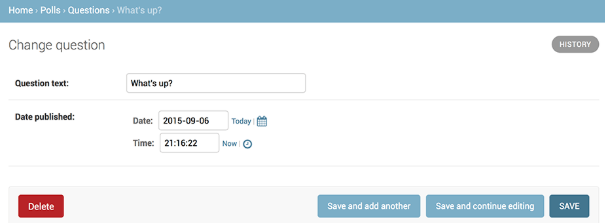
\includegraphics[scale=0.9]{figuras/3/32/325/img6.png}
\caption{Modificando la Question}
\end{center}
\end{figure}

Acá debemos tener en cuenta que:

\begin{itemize}
\item 
El formulario se genera automáticamente a partir del modelo de Pregunta.

\item 
Los diferentes tipos de campo de modelo ({\href{https://docs.djangoproject.com/en/3.0/ref/models/fields/\#django.db.models.DateTimeField}{\textcolor{B}{DateTimeField}}}, {\href{https://docs.djangoproject.com/en/3.0/ref/models/fields/\#django.db.models.CharField}{\textcolor{B}{CharField}}}
) corresponden al \textit{widget} de entrada \textbf{HTML} apropiado. Cada tipo de campo sabe cómo mostrarse en el administrador de \django{}.

\item
Cada {\href{https://docs.djangoproject.com/en/3.0/ref/models/fields/\#django.db.models.DateTimeField}{\textcolor{B}{DateTimeField}}} obtiene accesos directos de \textbf{JavaScript} gratuitos. Las fechas obtienen un acceso directo "Hoy" y una ventana emergente de calendario, y las horas obtienen un acceso directo "Ahora" y una ventana emergente conveniente que enumera las horas comúnmente ingresadas.


La parte inferior de la página le ofrece un par de opciones:

\item
Guardar: guarda los cambios y vuelve a la página de lista de cambios para este tipo de objeto.

\item
Guardar y continuar editando: guarda los cambios y vuelve a cargar la página de administración para este objeto.

\item
Guardar y agregar otro: guarda los cambios y carga un nuevo formulario en blanco para este tipo de objeto

\item
Eliminar: muestra una página de confirmación de eliminación

\end{itemize}


Si el valor de "Fecha de publicación" no coincide con la hora en que creó la pregunta en el Tutorial 1, probablemente significa que olvidó establecer el valor correcto para la configuración {\href{https://docs.djangoproject.com/en/3.0/ref/settings/\#std:setting-TIME\_ZONE}{\textcolor{B}{TIME\_ZONE}}}. Cámbielo, vuelva a cargar la página y verifique que aparezca el valor correcto.

Cambie la "Fecha de publicación" haciendo clic en los accesos directos "Hoy" y "Ahora". Luego haga clic en "Guardar y continuar editando". Luego haga clic en "Historial" en la esquina superior derecha. Verá una página que enumera todos los cambios realizados en este objeto a través del administrador de Django, con la marca de tiempo y el nombre de usuario de la persona que realizó el cambio:

\begin{figure}[H]
\begin{center}
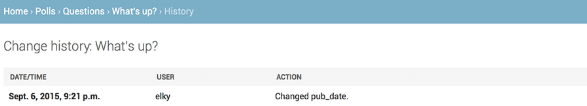
\includegraphics[scale=0.9]{figuras/3/32/325/img7.png}
\caption{Modificando la Question}
\end{center}
\end{figure}

Cuando se sienta cómodo con la API de modelos y se haya familiarizado con el sitio de administración, lea la {\href{https://docs.djangoproject.com/en/3.0/intro/tutorial03/}{\textcolor{B}{parte 3}}}  de este tutorial para obtener información sobre cómo agregar más vistas a nuestra aplicación de encuestas.

\subsection{Escribiendo tu primer aplicación con \django{}, parte 3}
\subsubsection{Visión general}

Una vista es un ``tipo'' de página web en su aplicación \django{} que generalmente cumple una función específica y tiene una plantilla específica. \textit{Por ejemplo}, en una aplicación de \textbf{blog}, puede tener las siguientes vistas:

\begin{itemize}
\item 
\textbf{HomePage del Blog} : 
Muestra las últimas entradas.

\item 
\textbf{Página de \textit{``detail''} de entrada} : página de enlace permanente para una sola entrada.

\item
\textbf{Página de archivo basada en el año} : muestra todos los meses con entradas en el año dado.
\item
\textbf{Página de archivo basada en el mes} : muestra todos los días con entradas en el mes dado.

\item
\textbf{Página de archivo basada en el día} : muestra todas las entradas en el día dado.

\item 
\textbf{Acción de comentario} : maneja la publicación de comentarios en una entrada determinada.
\end{itemize}

En nuestra aplicación de encuesta, tendremos las siguientes cuatro vistas:

\begin{itemize}
\item
\textbf{Página de \textit{``índice''} (index ) de preguntas}: muestra las últimas preguntas.

\item
\textbf{Página de \textit{``detalles''} (detail) de la pregunta} : muestra un texto de pregunta, sin resultados pero con un formulario para votar.

\item
\textbf{Página de \textit{``resultados''} (result) de la pregunta} :
Muestra un resultado para cada Question en particular.

\item
\textbf{Accion de voto} :
maneja la votación de una elección particular en una pregunta particular.
\end{itemize}

En \django{}, las páginas web y otros contenidos se entregan mediante vistas. Cada vista está representada por una función de \py{} (o método, en el caso de vistas basadas en clases). \django{} elegirá una vista examinando la \textbf{URL} solicitada (para ser precisos, la parte de la \textbf{URL} después del nombre de dominio).
\\\\
Ahora, en su tiempo en la web, puede haber encontrado cositas lindas como\\ \textit{"ME2/Sites/dirmod.asp?Sid=\&type=gen\&mod=Core+Pages\&gid=A6CD4967199A42D9B65B1B"}. \\Te complacerá saber que \django{} nos permite patrones de \textbf{URL} mucho más elegantes que eso.
\\\\
Un patrón de \textbf{URL} es la forma general de una \textbf{URL}, por ejemplo: \textbf{/newsarchive/$<$año$>$/$<$mes$>$/.}
\\\\
Para pasar de una \textbf{URL} a una vista, \django{} utiliza lo que se conoce como \textbf{``URLconfs''}. Un \textbf{URLconf} asigna patrones de \textbf{URL} a vistas.

Este tutorial proporciona instrucciones básicas sobre el uso de \textbf{URLconfs}, y puede consultar en {\href{https://docs.djangoproject.com/en/3.0/topics/http/urls/}{\textcolor{B}{URL info}}} para obtener más información.
\newpage

\subsubsection{Escribiendo más vistas}
Ahora, agreguemos unas vistas más a \textbf{polls/viwes.py}.
Estas vistas seran ligeramente diferentes, pues estas tomaran el \textit{id} de una \textbf{Question} como argumento ademas de el parametro obligatorio \textit{request}:

\begin{figure}[H]
\begin{center}
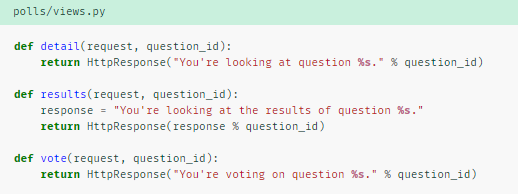
\includegraphics[scale=1]{figuras/3/33/332/img1.png}
\caption{Agregamos vistas}
\end{center}
\end{figure}

Instala estas nuevas vistas en el modulo \textbf{polls/urls}
agregando los siguientes {\href{https://docs.djangoproject.com/en/3.0/ref/urls/\#django.urls.path}{\textcolor{B}{path()}}}

\begin{figure}[H]
\begin{center}
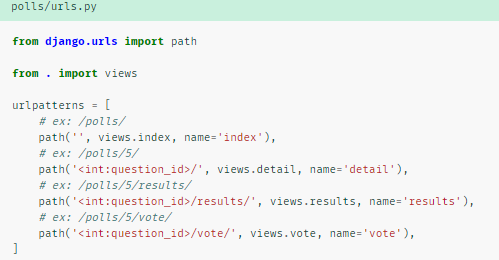
\includegraphics[scale=1]{figuras/3/33/332/img2.png}
\caption{Agregamos vistas}
\end{center}
\end{figure}

Eche un vistazo en su navegador, en \textbf{``/polls/34/''}. Ejecutará el método \textbf{detail()} y mostrará cualquier ID que proporciones en la \textbf{URL}. Pruebe \textbf{``/polls/34/results/''} y \textbf{``/polls/34/vote/''}  también; estos mostrarán los resultados de marcador de posición y las páginas de votación.

Cuando alguien solicita una página de su sitio web, por ejemplo, \textbf{``/polls/34/''}, \django{} cargará el módulo de \textit{Python mysite.urls} porque está indicado por la configuración \textbf{ROOT\_URLCONF}. Encuentra la variable llamada \textit{urlpatterns} y atraviesa los patrones en orden. Después de encontrar la coincidencia en \textbf{'polls/'}, elimina el texto coincidente (\textbf{"polls/"}) y envía el texto restante \textbf{-"34/"-} a la \textbf{URLconf} "\textit{polls.urls}" para su posterior procesamiento. Allí coincide con \textcolor{G}{'$<$int: question\_id$>$/'}, lo que resulta en una llamada a la vista de \textbf{detail()} así:

\begin{center}
\fbox{detail(request=$<$HttpRequest object$>$, question\_id=34)}
\end{center}

La parte \textit{question\_id} = 34 proviene de $<$int: question\_id$>$. El uso de corchetes angulares "captura" parte de la URL y la envía como argumento de palabra clave a la función de vista. La parte: \textit{question\_id}$>$ de la cadena define el nombre que se utilizará para identificar el patrón coincidente, y la \textit{$<$int: part} es un convertidor que determina qué patrones deben coincidir con esta parte de la ruta \textbf{URL}.

No es necesario agregar \textbf{URL cruft} como .\textbf{html}, a menos que lo desee, en cuyo caso puede hacer algo como esto:

$$\fbox{path('polls/latest.html', views.index),}$$

Pero no hagas eso, no es ni necesario ni comodo a la vista.

\subsubsection{Escribiendo vistas que realmente hacen algo}
Cada vista es responsable de hacer una de dos cosas: devolver un objeto {\href{https://docs.djangoproject.com/en/3.0/ref/request-response/\#django.http.HttpResponse}{\textcolor{B}{HttpResponse}}}
 que contenga el contenido de la página solicitada, o generar una excepción como {\href{https://docs.djangoproject.com/en/3.0/topics/http/views/\#django.http.Http404}{\textcolor{B}{Http404}}}
. El resto depende de usted


Su vista puede leer registros de una base de datos, o no. Puede usar un sistema de plantillas como el de \django{}, o un sistema de plantillas \py{} de terceros, o no. Puede generar un archivo \textbf{PDF}, generar \textbf{XML}, crear un archivo \textbf{ZIP} sobre la marcha, lo que desee, utilizando las bibliotecas de \py{} que desee.

Todo lo que \django{} quiere es que {\href{https://docs.djangoproject.com/en/3.0/ref/request-response/\#django.http.HttpResponse}{\textcolor{B}{HttpResponse}}}. O una excepción.

Debido a que es conveniente, usemos la propia \textbf{API} de base de datos de \django{}, que cubrimos en la \textit{parte 2}. Aquí hay una puñalada en una nueva vista de \textit{índice()}, que muestra las últimas 5 preguntas de encuesta en el sistema, separadas por comas, según la fecha de publicación

\begin{figure}[H]
\begin{center}
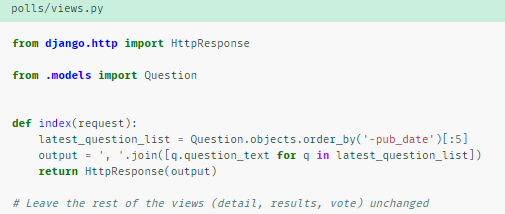
\includegraphics[scale=1]{figuras/3/33/333/img1.png}
\caption{Modificamos la función \textit{index}}
\end{center}
\end{figure}


Sin embargo, hay un problema aquí: el diseño de la página está codificado en la vista. Si desea cambiar el aspecto de la página, deberá editar este código de \py{}. Entonces, usemos el sistema de plantillas de \django{} para separar el diseño de \py{} creando una plantilla que la vista pueda usar.


Primero, cree un directorio llamado plantillas en su directorio de encuestas. \django{} buscará plantillas allí.

La configuración de \textbf{TEMPLATES} (plantillas) de su proyecto describe cómo \django{} cargará y renderizará las plantillas. El archivo de configuración predeterminado configura un \textit{back-end} de \textcolor{G}{DjangoTemplates} cuya opción \textcolor{G}{APP\_DIRS} está establecida en \textcolor{R}{True}. Por convención, \textcolor{G}{DjangoTemplates} busca un subdirectorio de "plantillas" en cada una de las \textcolor{G}{INSTALLED\_APPS}.


Dentro del directorio de plantillas que acaba de crear, cree otro directorio llamado encuestas, y dentro de ese, cree un archivo llamado \textit{index.html}. En otras palabras, su plantilla debe estar en \textbf{polls/templates/polls/index.html}. Debido a cómo funciona el cargador de plantillas \textcolor{G}{app\_directories} como se describe anteriormente, puede referirse a esta plantilla dentro de \django{} como \textbf{polls/index.html}.


\begin{table}[H]
	%\renewcommand{\arraystretch}{1.3}	
	\begin{tabular}{||c||}
	\hline \\
	\begin{Large}
	\textbf{\textit{
Espacio de nombres de plantillas (\textit{Template namespacing})}}
	\end{Large}
	\\\\		
Ahora podríamos evitar poner nuestras plantillas directamente en \textbf{polls/templates}\\ (en lugar de crear otro subdirectorio de encuestas), pero en realidad sería una mala idea.\\ \django{} elegirá la primera plantilla que encuentre cuyo nombre coincida, y si tuviera\\ una plantilla con el mismo nombre en una aplicación diferente, \django{} no podría distinguir entre ellas.\\ Necesitamos poder apuntar a \django{} al correcto, y la mejor manera de asegurar esto es espaciando los nombres.\\ Es decir, colocando esas plantillas dentro de otro directorio nombrado para la aplicación misma.
\\\\ \hline 	
			\end{tabular}
		\end{table}		

Pon el siguiente código en esa plantilla:

\begin{figure}[H]
\begin{center}
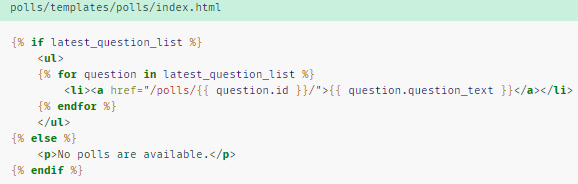
\includegraphics[scale=1]{figuras/3/33/333/img2.png}
\caption{Modificamos la función \textit{index}}
\end{center}
\end{figure}

\begin{table}[H]
	%\renewcommand{\arraystretch}{1.3}	
	\begin{tabular}{||c||}
	\hline \\
	\begin{Large}
	\textbf{Nota}
	\end{Large}
	\\\\		
	
Para acortar el tutorial, todos los ejemplos de plantillas usan HTML incompleto.\\ En sus propios proyectos, debe usar {\href{https://developer.mozilla.org/en-US/docs/Learn/HTML/Introduction_to_HTML/Getting_started#Anatomy_of_an_HTML_document}{\textcolor{B}{documentos HTML completos}}}.
\\\\ \hline 	
			\end{tabular}
		\end{table}		

Ahora actualicemos nuestro \textit{index} en \textbf{polls/views.py} para que use el la platnilla \textit{index.html}

\begin{figure}[H]
\begin{center}
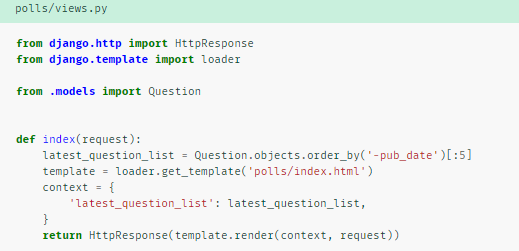
\includegraphics[scale=1]{figuras/3/33/333/img3.png}
\caption{Agregamos el \textit{loader} para cargar el \textit{template} en la función \textit{index}}
\end{center}
\end{figure}

Ese código carga la plantilla llamada \textit{polls/index.html} y le pasa un contexto. El contexto es una plantilla de mapeo de diccionario de nombres de variables a objetos de \py{}.


Cargue la página apuntando su navegador a "\textbf{/polls/}", y debería ver una lista con viñetas que contiene la pregunta "¿Qué pasa?" en la \textit{parte 2}. El enlace apunta a la página de detalles de la pregunta.

\subsubsection*{Otra forma es renderisar ({\href{https://docs.djangoproject.com/en/3.0/topics/http/shortcuts/\#django.shortcuts.render}{\textcolor{B}{shourcat render()}}})}

Existe una forma muy común cargar una plantilla, llenar un contexto y devolver un objeto {\href{https://docs.djangoproject.com/en/3.0/ref/request-response/\#django.http.HttpResponse}{\textcolor{B}{HttpResponse}}} con el resultado de la plantilla renderizada. Django proporciona un acceso directo. Aquí está la vista completa del índice (), reescrita:

\begin{figure}[H]
\begin{center}
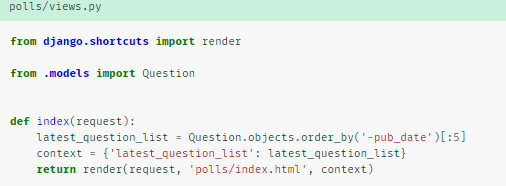
\includegraphics[scale=1]{figuras/3/33/333/img4.png}
\caption{Agregamos el \textit{loader} para cargar el \textit{template} en la función \textit{index}}
\end{center}
\end{figure}

Tenga en cuenta que una vez que hayamos hecho esto en todas estas vistas, ya no necesitamos importar el cargador ({\href{https://docs.djangoproject.com/en/3.0/topics/templates/\#module-django.template.loader}{\textcolor{B}{loader}}}) y {\href{https://docs.djangoproject.com/en/3.0/ref/request-response/\#django.http.HttpResponse}{\textcolor{B}{HttpResponse}}} (querrá mantener {\href{https://docs.djangoproject.com/en/3.0/ref/request-response/\#django.http.HttpResponse}{\textcolor{B}{HttpResponse}}} si todavía tiene los métodos de código auxiliar para obtener detalles, resultados y votar).

La función {\href{https://docs.djangoproject.com/en/3.0/topics/http/shortcuts/#django.shortcuts.render}{\textcolor{B}{render()}}} toma el objeto de solicitud como su primer argumento, un nombre de plantilla como su segundo argumento y un diccionario como su tercer argumento opcional. Devuelve un objeto {\href{https://docs.djangoproject.com/en/3.0/ref/request-response/\#django.http.HttpResponse}{\textcolor{B}{HttpResponse}}} de la plantilla dada representada con el contexto dado.

\subsubsection{Errores 404}

Ahora, abordemos la vista detallada de la pregunta: la página que muestra el texto de la pregunta para una encuesta determinada. Aquí está la vista:

\begin{figure}[H]
\begin{center}
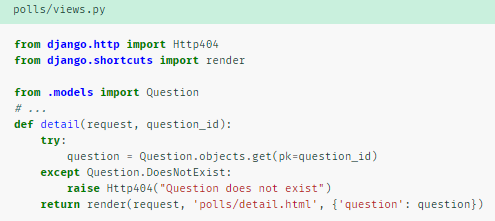
\includegraphics[scale=1]{figuras/3/33/334/img1.png}
\caption{Levantamiento de un Error 404 sobre el view}
\end{center}
\end{figure}


El nuevo concepto aquí: la vista genera (\textit{raise}) la excepción {\href{https://docs.djangoproject.com/en/3.0/topics/http/views/\#django.http.Http404}{\textcolor{B}{Http404}}}
 si no existe una pregunta con el \textbf{ID} solicitado.

Discutiremos un poco más adelante qué podría poner en esa plantilla de \textbf{polls/detail.html}, pero si desea que el ejemplo anterior funcione rápidamente, un archivo que contiene solo:

\begin{figure}[H]
\begin{center}
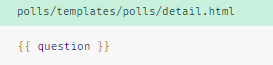
\includegraphics[scale=1]{figuras/3/33/334/img2.png}
\caption{template del \textit{detail.html}}
\end{center}
\end{figure}

\subsubsection*{Shortcut: \textcolor{R}{get\_object\_or\_404()}}
Es muy común utilizar  un  {\href{https://docs.djangoproject.com/en/3.0/ref/models/querysets/\#django.db.models.query.QuerySet.get}{\textcolor{B}{get()}}} para generar un {\href{https://docs.djangoproject.com/en/3.0/topics/http/views/\#django.http.Http404}{\textcolor{B}{Http404}}} si es que el objeto no existe en la base de datos. \django{} provee un \textit{shortcut} para este tipo de cosas, este es el {\href{https://docs.djangoproject.com/en/3.0/topics/http/shortcuts/\#django.shortcuts.get\_object\_or\_404}{\textcolor{B}{get\_object\_or\_404()}}}. El codigo utilizando esta herramienta nos quedaria como sigue:

\begin{figure}[H]
\begin{center}
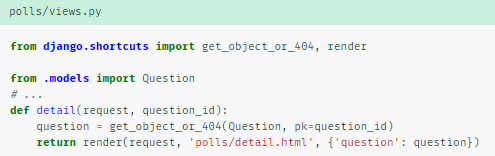
\includegraphics[scale=1]{figuras/3/33/334/img3.png}
\caption{Funcion detail}
\end{center}
\end{figure}


La función {\href{https://docs.djangoproject.com/en/3.0/topics/http/shortcuts/\#django.shortcuts.get\_object\_or\_404}{\textcolor{B}{get\_object\_or\_404()}}} toma un \textit{\django{} model} como primer argumento 
y un número arbitrario de argumentos de palabras clave, que pasa a la función {\href{https://docs.djangoproject.com/en/3.0/ref/models/querysets/\#django.db.models.query.QuerySet.get}{\textcolor{B}{get()}}} del administrador del modelo.
Si el modelo no existe genera un {\href{https://docs.djangoproject.com/en/3.0/topics/http/views/\#django.http.Http404}{\textcolor{B}{Http404}}}.

\begin{table}[H]
	%\renewcommand{\arraystretch}{1.3}	
	\begin{tabular}{||c||}
	\hline \\
	\begin{Large}
	\textbf{Filosofia}
	\end{Large}
	\\\\		
¿Por qué utilizamos una función auxiliar {\href{https://docs.djangoproject.com/en/3.0/topics/http/shortcuts/\#django.shortcuts.get\_object\_or\_404}{\textcolor{B}{get\_object\_or\_404()}}} en lugar de detectar\\ automáticamente las excepciones {\href{https://docs.djangoproject.com/en/3.0/ref/exceptions/\#django.core.exceptions.ObjectDoesNotExist}{\textcolor{B}{ObjectDoesNotExist}}} en un nivel superior,\\ o hacer que la API del modelo genere {\href{https://docs.djangoproject.com/en/3.0/topics/http/views/\#django.http.Http404}{\textcolor{B}{Http404}}} en lugar de {\href{https://docs.djangoproject.com/en/3.0/ref/exceptions/\#django.core.exceptions.ObjectDoesNotExist}{\textcolor{B}{ObjectDoesNotExist}}}?\\

Porque eso acoplaría la capa del modelo a la capa de vista.\\ Uno de los principales objetivos de diseño de \django{} es mantener un acoplamiento flexible.\\ Se introduce algún acoplamiento controlado en el módulo \textcolor{G}{django.shortcuts}.
\\\\ \hline 	
			\end{tabular}			
		\end{table}		

También hay una función {\href{https://docs.djangoproject.com/en/3.0/topics/http/shortcuts/\#django.shortcuts.get\_list\_or\_404}{\textcolor{B}{get\_list\_or\_404()}}}, que funciona igual que {\href{https://docs.djangoproject.com/en/3.0/topics/http/shortcuts/\#django.shortcuts.get\_object\_or\_404}{\textcolor{B}{get\_object\_or\_404()}}}, excepto que usa {\href{https://docs.djangoproject.com/en/3.0/ref/models/querysets/\#django.db.models.query.QuerySet.filter}{\textcolor{B}{filter()}}} en lugar de {\href{https://docs.djangoproject.com/en/3.0/ref/models/querysets/\#django.db.models.query.QuerySet.get}{\textcolor{B}{get()}}}. Eleva {\href{https://docs.djangoproject.com/en/3.0/topics/http/views/\#django.http.Http404}{\textcolor{B}{Http404}}} si la lista está vacía.			
			
\subsubsection{Usando el sistema de plantillas}

Volviendo a la visata del \textit{detail}  para nuestra aplicación de encuestas. Dada la pregunta de la variable de contexto, así es como se vería la plantilla \textbf{polls/detail.html}:

\begin{figure}[H]
\begin{center}
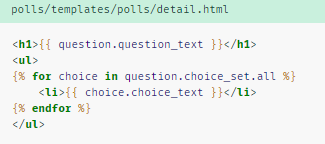
\includegraphics[scale=1]{figuras/3/33/335/img1.png}
\caption{template del \textit{detail.html}}
\end{center}
\end{figure}

El sistema de plantillas utiliza la sintaxis de búsqueda de puntos para acceder a los atributos variables. En el ejemplo de \textcolor{R}{ \{\{ question.question\_text \}\} }, primero \django{} realiza una búsqueda de diccionario en la pregunta del objeto. De lo contrario, intenta una búsqueda de atributos, que en este caso, funciona. Si la búsqueda de atributos hubiera fallado, habría intentado una búsqueda de índice de lista.


La llamada al metodo ocurre en el bucle \textbf{\{\{\% for \%\}\}}: \textcolor{R}{ question.choice\_set.all } se interpreta como el código \py{} \textcolor{G}{ question.choice\_set.all() }, que devuelve un iterable de objetos \textbf{Choice} y se itera con un \textbf{\{\{\% for \%\}\}}.

En la {\href{https://docs.djangoproject.com/en/3.0/topics/templates/}{\textcolor{B}{Guia de templates}}} vas a encontrar más info.


\subsubsection{Eliminando URLs codificadas en plantillas}

Recordemos, cuando escribimos el link hacia el template \textbf{polls/index.hml}, el link estaba codificado (hardcodeado) masomenos así:

\begin{figure}[H]
\begin{center}
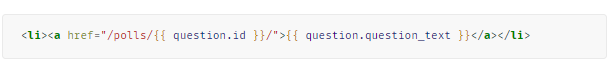
\includegraphics[scale=1]{figuras/3/33/336/img1.png}
%\caption{template del \textit{detail.html}}
\end{center}
\end{figure}

El problema con esta codificación aproximada es que se convierte en un desafío cambiar las \textbf{URL} en proyectos con muchas plantillas. Sin embargo, dado que definió el argumento de nombre en las funciones {\href{https://docs.djangoproject.com/en/3.0/ref/urls/\#django.urls.path}{\textcolor{B}{path()}}}
 en el módulo \textcolor{G}{polls.urls}, puede eliminar la dependencia de rutas \textbf{URL} específicas definidas en sus configuraciones de \textbf{URL} utilizando la etiqueta de plantilla \{\% url \%\}:

\begin{figure}[H]
\begin{center}
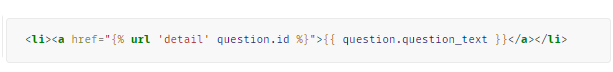
\includegraphics[scale=1]{figuras/3/33/336/img2.png}
%\caption{template del \textit{detail.html}}
\end{center}
\end{figure}


La forma en que esto funciona es buscando la definición de \textbf{URL} como se especifica en el módulo \textcolor{G}{polls.urls}. Puede ver exactamente dónde se define a continuación el nombre de \textbf{URL} de \textit{"detail"}

\begin{figure}[H]
\begin{center}
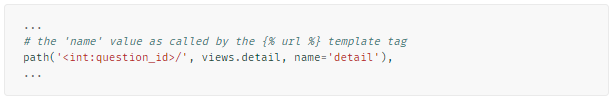
\includegraphics[scale=1]{figuras/3/33/336/img3.png}
%\caption{template del \textit{detail.html}}
\end{center}
\end{figure}

Si desea cambiar la \textbf{URL} de la vista de detalles de las encuestas a otra, tal vez a algo como \textbf{polls/detail/12/} en lugar de hacerlo en la plantilla (o plantillas), debe cambiarla en \textbf{polls/urls.py}:

\begin{figure}[H]
\begin{center}
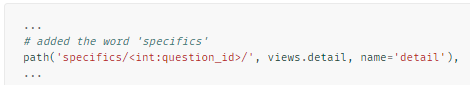
\includegraphics[scale=1]{figuras/3/33/336/img4.png}
%\caption{template del \textit{detail.html}}
\end{center}
\end{figure}

\subsubsection{Namespacing URL}
El proyecto tiene solo una aplicación, \textit{polls}. En proyectos reales de \django{}, puede haber cinco, diez, veinte aplicaciones o más. \textit{¿Cómo diferencia Django los nombres de URL entre ellos?} Por ejemplo, la aplicación de encuestas tiene una vista detallada, y también podría tener una aplicación en el mismo proyecto que es para un \textbf{blog}. \textit{¿Cómo se logra que \django{} sepa qué vista de aplicación crear para una \textbf{URL} cuando se usa la etiqueta de plantilla \{\% url \%\}?}

La respuesta es \textit{agregar namespaces} al \textbf{URLconf} en \textbf{polls/urls.py}. Para esto vamos a \textbf{polls/urls.py} y agregamos la variable \textbf{app\_name} para setear el namespace de la aplicación:

\begin{figure}[H]
\begin{center}
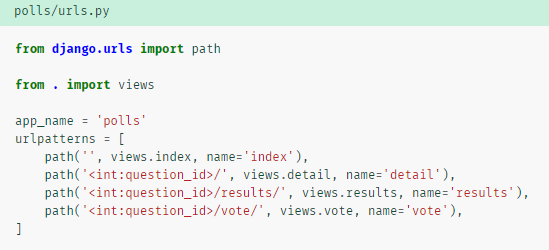
\includegraphics[scale=1]{figuras/3/33/337/img1.png}
\caption{Agregamos el namespace a \textbf{polls/urls.py}}
\end{center}
\end{figure}

Luego, modificamos el template del index de la siguiente forma:

\begin{figure}[H]
\begin{center}
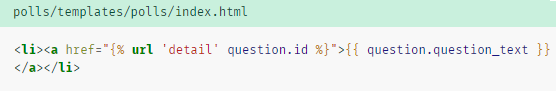
\includegraphics[scale=1]{figuras/3/33/337/img2.png}
\caption{Agregamos el namespace a \textbf{polls/urls.py}}
\end{center}
\end{figure}

y para apuntar al namespace de la vista del detail:

\begin{figure}[H]
\begin{center}
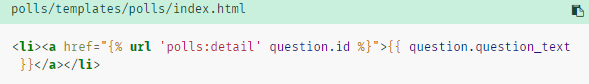
\includegraphics[scale=1]{figuras/3/33/337/img3.png}
\caption{Agregamos el namespace a \textbf{polls/urls.py}}
\end{center}
\end{figure}

\newpage
\subsection{Escribiendo tu primer aplicación en \django{}, parte 4}
\subsubsection{Escribiendo un pequeño formulario}

Actualicemos nuestra plantilla de detalles de la encuesta (\textbf{polls/detail.html}) del último tutorial, de modo que la plantilla contenga un elemento \textbf{HTML} \textcolor{G}{$<$form$>$}:

\begin{figure}[H]
\begin{center}
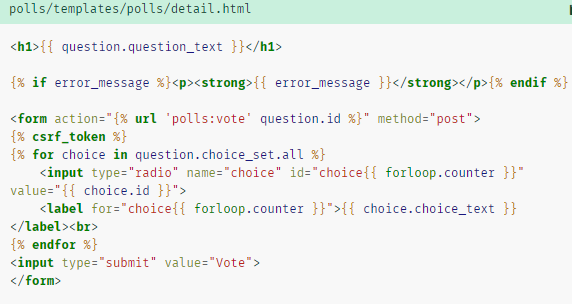
\includegraphics[scale=1]{figuras/3/34/341/img1.png}
\caption{Agregamos el namespace a \textbf{polls/urls.py}}
\end{center}
\end{figure}

Resumiendo:
\begin{itemize}
\item 
La plantilla anterior muestra un botón de opción para cada elección de pregunta. El valor de cada botón de opción es la ID de la opción de pregunta asociada. El nombre de cada botón de radio es \textbf{"Choice"}. Eso significa que, cuando alguien selecciona uno de los botones de opción y envía el formulario, enviará la opción \textbf{POST} de \textbf{Choice=\#} donde \# es el ID de la opción seleccionada. Este es el concepto básico de los formularios \textbf{HTML}.

\item
Establecemos la acción del formulario en \textcolor{R}{\{\% url 'polls:vote' question.id \%\}}, y configuramos \textit{method = "post"}. Usar \textit{method = "post"} (en oposición a \textit{method = "get"}) es muy importante, \textbf{porque el acto de enviar este formulario alterará los datos del lado del servidor}. Siempre que cree un formulario que altere el lado del servidor de datos, use \textit{method = "post"}. Este consejo no es específico de \django{}; es una buena práctica de desarrollo web en general.

\item
\textcolor{G}{forloop.counter} indica cuántas veces la etiqueta {\href{https://docs.djangoproject.com/en/3.0/ref/templates/builtins/\#std:templatetag-for}{\textcolor{B}{for}}} ha pasado por su bucle
\item
Dado que estamos creando un formulario \textbf{POST} (que puede tener el efecto de modificar los datos), debemos preocuparnos por \textit{las falsificaciones de solicitudes de sitios cruzados}. Afortunadamente, no debemos preocuparnos demasiado, porque \django{} viene con un sistema útil para protegernos de esto. En resumen, todos los formularios \textbf{POST} que están dirigidos a las \textbf{URL} internas deben usar la etiqueta de plantilla\\ {\href{https://docs.djangoproject.com/en/3.0/ref/templates/builtins/\#std:templatetag-csrf_token}{\textcolor{B}{\{\% csrf\_token \%\} }}}.
\end{itemize}

Ahora, creemos una vista que maneje los datos enviados y haga algo con ellos. Recuerde, en la parte 3, creamos una \textbf{URLconf} para la aplicación de encuestas que incluye esta línea:

\begin{figure}[H]
\begin{center}
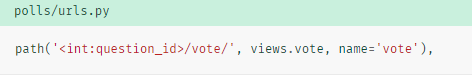
\includegraphics[scale=1]{figuras/3/34/341/img2.png}
\caption{Agregamos el namespace a \textbf{polls/urls.py}}
\end{center}
\end{figure}

También creamos una implementación ficticia de la función \textit{vote()}. Vamos a crear una versión que sirva de algo. Agreguemos lo siguiente a \textbf{polls/views.py}:

\begin{figure}[H]
\begin{center}
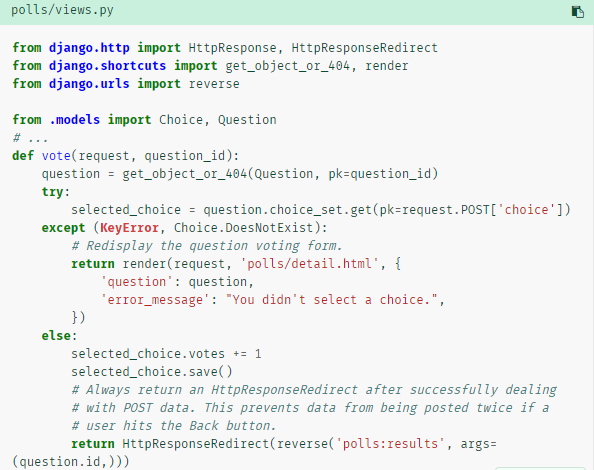
\includegraphics[scale=1]{figuras/3/34/341/img3.png}
\caption{Agregamos el namespace a \textbf{polls/urls.py}}
\end{center}
\end{figure}

Este código incluye algunas cosas que aún no hemos cubierto en hasta ahora:

\begin{itemize}
\item
{\href{https://docs.djangoproject.com/en/3.0/ref/request-response/\#django.http.HttpRequest.POST}{\textcolor{B}{request.POST}}}
 es un objeto similar a un diccionario que le permite acceder a los datos enviados por nombre de clave. En este caso, \textcolor{G}{request.POST}\textcolor{R}{['choice']} devuelve el \textbf{ID} de la opción seleccionada, como una cadena. {\href{https://docs.djangoproject.com/en/3.0/ref/request-response/\#django.http.HttpRequest.POST}{\textcolor{B}{request.POST}}}
 valores son siempre cadenas.

Tenga en cuenta que \django también proporciona {\href{https://docs.djangoproject.com/en/3.0/ref/request-response/\#django.http.HttpRequest.GET}{\textcolor{B}{request.GET}}} para acceder a los datos \textbf{GET} de la misma manera, pero estamos usando explícitamente {\href{https://docs.djangoproject.com/en/3.0/ref/request-response/\#django.http.HttpRequest.POST}{\textcolor{B}{request.POST}}} en nuestro código, para garantizar que los datos solo se modifiquen a través de una llamada \textbf{POST}.

\item
\textcolor{G}{request.POST}\textcolor{R}{['choice']} generará {\href{https://docs.python.org/3/library/exceptions.html\#KeyError}{\textcolor{B}{KeyError}}} si la elección no se proporcionó en los datos \textbf{POST}. El código anterior verifica {\href{https://docs.python.org/3/library/exceptions.html\#KeyError}{\textcolor{B}{KeyError}}} y vuelve a mostrar el formulario de pregunta con un mensaje de error si no se da la opción.

\item
Después de incrementar el recuento de opciones, el código devuelve un {\href{https://docs.djangoproject.com/en/3.0/ref/request-response/\#django.http.HttpResponseRedirect}{\textcolor{B}{HttpResponseRedirect}}} en lugar de un {\href{https://docs.djangoproject.com/en/3.0/ref/request-response/\#django.http.HttpResponse}{\textcolor{B}{HttpResponse}}} normal. {\href{https://docs.djangoproject.com/en/3.0/ref/request-response/\#django.http.HttpResponseRedirect}{\textcolor{B}{HttpResponseRedirect}}} toma un solo argumento: la \textbf{URL} a la que se redirigirá al usuario (consulte el siguiente punto para ver cómo construimos la \textbf{URL} en este caso).

Como señala el comentario de \py{} anterior, siempre debe devolver un {\href{https://docs.djangoproject.com/en/3.0/ref/request-response/\#django.http.HttpResponseRedirect}{\textcolor{B}{HttpResponseRedirect}}} después de tratar con éxito los datos \textbf{POST}. Este consejo no es específico de \django{}; es una buena práctica de desarrollo web en general.

\item
Estamos utilizando la función \textit{reverse()} en el constructor {\href{https://docs.djangoproject.com/en/3.0/ref/request-response/\#django.http.HttpResponseRedirect}{\textcolor{B}{HttpResponseRedirect}}} en este ejemplo. Esta función ayuda a evitar tener que codificar una \textbf{URL} en la función de vista. Se le da el nombre de la vista a la que queremos pasar el control y la parte variable del patrón de \textbf{URL} que apunta a esa vista. En este caso, usando la \textbf{URLconf} que configuramos en la parte 3, esta llamada \textit{reverse()} devolverá una cadena como

\begin{figure}[H]
\begin{center}
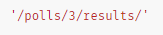
\includegraphics[scale=1]{figuras/3/34/341/img4.png}
%\caption{Agregamos el namespace a \textbf{polls/urls.py}}
\end{center}
\end{figure}
Donde el \textbf{3} es el valor de \textcolor{G}{question.id}
Esta redireccion del URL llamara a la vista \textit{'results'}
para mostrar (display) la pagina final. 

\end{itemize}

Como se mencionó en la parte 3, la solicitud es un objeto {\href{https://docs.djangoproject.com/en/3.0/ref/request-response/\#django.http.HttpRequest}{\textcolor{B}{HttpRequest}}}
. Para obtener más información sobre los objetos {\href{https://docs.djangoproject.com/en/3.0/ref/request-response/\#django.http.HttpRequest}{\textcolor{B}{HttpRequest}}}
, {\href{https://docs.djangoproject.com/en/3.0/ref/request-response/}{\textcolor{B}{consulte la documentación de solicitud y respuesta}}}


Después de que alguien vota en una pregunta, la vista vote () redirige a la página de resultados de la pregunta. Escribamos esa vista:


\begin{figure}[H]
\begin{center}
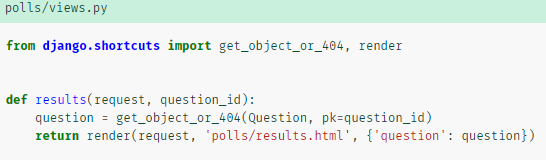
\includegraphics[scale=1]{figuras/3/34/341/img5.png}
%\caption{Agregamos el namespace a \textbf{polls/urls.py}}
\end{center}
\end{figure}

Esto es casi exactamente lo mismo que la vista de \textit{detail()}. La única diferencia es el nombre de la plantilla. Arreglaremos esta redundancia más tarde.

Ahora, creemos una plantilla de resultados en \textbf{polls/templates/polls/result.html} 

\begin{figure}[H]
\begin{center}
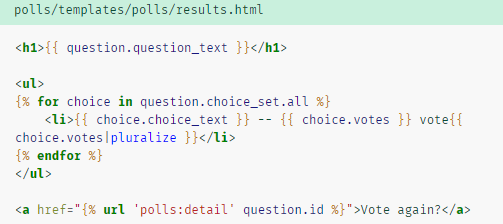
\includegraphics[scale=0.9]{figuras/3/34/341/img6.png}
%\caption{Agregamos el namespace a \textbf{polls/urls.py}}
\end{center}
\end{figure}


Ahora, vaya a \textbf{/polls/1/} en su navegador y vote en la pregunta. Debería ver una página de resultados que se actualiza cada vez que vota. Si envía el formulario sin haber elegido una opción, debería ver un mensaje de error.

\begin{small}
\begin{table}[H]
	%\renewcommand{\arraystretch}{1.3}	
	\begin{tabular}{||c||}
	\hline \\
	\begin{Large}
	\textbf{Nota}
	\end{Large}
	\\	
El código para nuestra vista \textit{vote()} tiene un pequeño problema.\\ Primero obtiene el objeto \textcolor{G}{selected\_choice} de la base de datos, luego calcula el nuevo valor de los votos\\ y luego lo guarda de nuevo en la base de datos.\\ Si dos usuarios de su sitio web intentan votar exactamente al mismo tiempo,\\ esto podría salir mal: el mismo valor, digamos 42, se recuperará para los votos.\\ Luego, para ambos usuarios se calcula y guarda el nuevo valor de 43, pero 44 sería el valor esperado.\\

Esto se llama condición de carrera. Si está interesado,\\ puede leer {\href{https://docs.djangoproject.com/en/3.0/ref/models/expressions/#avoiding-race-conditions-using-f}{\textcolor{B}{Evitar condiciones de carrera usando \textbf{F()}}}} para aprender cómo puede resolver este problema.
\\ \hline 	
			\end{tabular}			
		\end{table}		
\end{small}
\subsubsection{Vistas Genéricas (Cuanto menos código, mejor!)}
Las vistas \textit{detail()} y \textit{results()} son bastante cortas y ademas redundantes.
La vista \textit{index()}, que muestra una lista de encuestas, es similar.

Estas vistas representan un caso común de desarrollo web básico: obtener datos de la base de datos de acuerdo con un parámetro pasado en la \textbf{URL}, cargar una plantilla y devolver la plantilla representada. Como esto es tan común, \django{} proporciona un acceso directo, llamado sistema de ``vistas genéricas''.

Las vistas genéricas resumen patrones comunes hasta el punto en que ni siquiera necesita escribir código \py{} para escribir una aplicación.

Convirtamos nuestra aplicación de encuestas para usar el sistema de vistas genéricas, para que podamos eliminar un montón de nuestro propio código. Tendremos que seguir algunos pasos para realizar la conversión:

\begin{itemize}
\item Modificar \textbf{URLconf}
\item Eliminar las viejas vistas
\item Introducir las vistas genéricas aportadas por \django{}
\end{itemize}


\begin{table}[H]	
	\begin{tabular}{||c||}
		\hline \\
		\begin{Large}
			\textbf{¿Porque la evación de código?}
		\end{Large}
		\\		
En general, al escribir una aplicación \django{}, evaluará si las vistas genéricas son adecuadas\\ para su problema y las usará desde el principio, en lugar de refactorizar\\ su código a la mitad.\\ Pero este tutorial se ha centrado intencionalmente en escribir las vistas \\``por el camino difícil'' hasta ahora, para centrarse en los conceptos básicos.\\\\

Debe conocer las matemáticas básicas antes de comenzar a usar una calculadora.
		\\ \hline 	
	\end{tabular}			
\end{table}		

\subsubsection*{Modificar URLconf}
Abrimos \textbf{polls/urls.py} y modificamos los path de la siguiente manera:
\begin{figure}[H]
\begin{center}
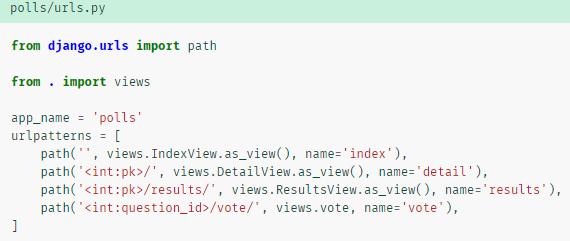
\includegraphics[scale=1]{figuras/3/34/342/img1.png}
%\caption{Agregamos el namespace a \textbf{polls/urls.py}}
\end{center}
\end{figure}
Notemos que el nombre patrón de la cadena de la ruta tanto del segundo, como del tercer path cambio de \textbf{$<$question\_id$>$} to \textbf{$<$pk$>$}. 
\subsubsection*{Modificar las vistas}
A continuación, vamos a eliminar nuestras vistas antiguas de índice, detalle y resultados y, en su lugar, utilizaremos las vistas genéricas de \django{}. Para hacerlo, abra el archivo \textbf{polls/views.py} y cámbielo así:
\begin{figure}[H]
\begin{center}
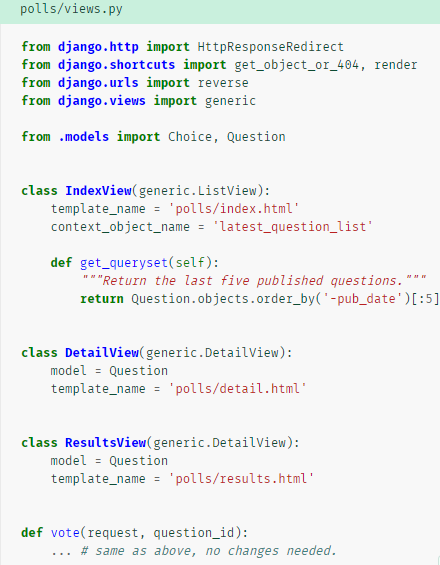
\includegraphics[scale=0.85]{figuras/3/34/342/img2.png}
%\caption{Agregamos el namespace a \textbf{polls/urls.py}}
\end{center}
\end{figure}

Aquí usamos dos vistas genéricas: {\href{https://docs.djangoproject.com/en/3.0/ref/class-based-views/generic-display/\#django.views.generic.list.ListView}{\textcolor{B}{ListView}}}
y
{\href{https://docs.djangoproject.com/en/3.0/ref/class-based-views/generic-display/\#django.views.generic.detail.DetailView}{\textcolor{B}{DetailView}}}
. Respectivamente, esas dos vistas resumen los conceptos de "mostrar una lista de objetos" y "mostrar una página de detalles para un tipo particular de objeto".

\begin{itemize}
\item 
Cada vista genérica necesita saber sobre qué modelo actuará. Esto se proporciona utilizando el atributo modelo.
\item
La vista genérica {\href{https://docs.djangoproject.com/en/3.0/ref/class-based-views/generic-display/\#django.views.generic.detail.DetailView}{\textcolor{B}{DetailView}}} espera que el valor de la clave principal capturado de la \textbf{URL} se llame \textbf{``pk''}, por lo que hemos cambiado \textbf{question\_id} a \textbf{pk} para las vistas genéricas.
\end{itemize}


Por defecto, la vista genérica {\href{https://docs.djangoproject.com/en/3.0/ref/class-based-views/generic-display/\#django.views.generic.detail.DetailView}{\textcolor{B}{DetailView}}} utiliza una plantilla llamada  \textbf{$<$app name$>$/$<$model name$>$\_detail.html}. En nuestro caso, usaría la plantilla \textbf{``polls/question\_detail.html''}. El atributo \textcolor{G}{template\_name} se usa para decirle a \django{} que use un nombre de plantilla específico en lugar del nombre de plantilla predeterminado autogenerado. También especificamos \textcolor{G}{template\_name} para la vista de la lista de resultados: esto garantiza que la vista de resultados y la vista de detalles tengan una apariencia diferente cuando se procesen, a pesar de que ambas son {\href{https://docs.djangoproject.com/en/3.0/ref/class-based-views/generic-display/\#django.views.generic.detail.DetailView}{\textcolor{B}{DetailView}}} detrás de escena.


Del mismo modo, la vista genérica {\href{https://docs.djangoproject.com/en/3.0/ref/class-based-views/generic-display/\#django.views.generic.list.ListView}{\textcolor{B}{ListView}}} utiliza una plantilla predeterminada llamada\textbf{$<$app name$>$/$<$model name$>$\_list.html}; usamos \textcolor{G}{template\_name} para decirle a {\href{https://docs.djangoproject.com/en/3.0/ref/class-based-views/generic-display/\#django.views.generic.list.ListView}{\textcolor{B}{ListView}}} que use nuestra plantilla existente \textbf{``polls/index.html''}.


En partes anteriores del tutorial, las plantillas han recibido un contexto que contiene las variables de contexto question y \textit{latest\_question\_list}. Para DetailView, la variable de pregunta se proporciona automáticamente, ya que estamos utilizando un modelo de Django (Pregunta), Django puede determinar un nombre apropiado para la variable de contexto. Sin embargo, para ListView, la variable de contexto generada automáticamente es \textit{question\_list}. Para anular esto, proporcionamos el atributo \textit{context\_object\_name}, especificando que queremos usar \textit{latest\_question\_list} en su lugar. Como un enfoque alternativo, puede cambiar sus plantillas para que coincidan con las nuevas variables de contexto predeterminadas, pero es mucho más fácil decirle a Django que use la variable que desee.

Ejecute el servidor y use su nueva aplicación de sondeo basada en vistas genéricas.

Para obtener detalles completos sobre vistas genéricas, consulte la {\href{https://docs.djangoproject.com/en/3.0/topics/class-based-views/}{\textcolor{B}{ documentación de vistas genéricas}}}.

\newpage
\subsection{Escribiendo tu primera aplicación \django{}, parte 5}
\subsubsection{Testing: Introduciendo pruebas automatizadas}
\subsubsection*{¿Qué son las pruebas automatizadas?}

Los test son rutinas que chequean si tu codigo opera de manera adecuada.

Las pruebas operan a diferentes niveles. Algunas pruebas pueden aplicarse a un pequeño detalle (\textit{¿un método de modelo en particular devuelve los valores esperados?}), mientras que otras examinan el funcionamiento general del software (\textit{¿produce una secuencia de entradas del usuario en el sitio el resultado deseado?}). Eso no es diferente del tipo de prueba que realizó anteriormente en la segunda parte, utilizando el \textit{shell} para examinar el comportamiento de un método, o ejecutando la aplicación e ingresando datos para verificar cómo se comporta.

La diferencia en las pruebas automatizadas es que el sistema realiza el trabajo de prueba por vos. Podes crear un conjunto de pruebas una vez, y después, a medida que realizas cambios en tu aplicación, podes verificar que tu código siga funcionando como querías , sin tener que realizar pruebas manuales que requieren mucho tiempo.

\subsubsection*{¿Porque tenemos que hacer tests?}
Quizas sientas que ya tenes ddemaciado aprendiendo \textbf{Python/Django}, y tener otra cosa más que aprender y hacer puede parecer abrumador y quizás innecesario. Después de todo, nuestra aplicación de encuestas está funcionando bastante bien ahora; pasar por el problema de crear pruebas automatizadas no va a hacer que funcione mejor. Si crear la aplicación de encuestas es la última parte de la programación de \django{} que harás, entonces es cierto, no necesitas saber cómo crear pruebas automatizadas. Pero, si ese no es el caso, ahora es un excelente momento para aprender.

\subsubsection*{\textit{Los Test pueden ahorrarte tiempo}}
Hasta cierto punto, "comprobar que parece funcionar" será una prueba satisfactoria. En una aplicación más sofisticada, puede tener docenas de interacciones complejas entre componentes.


Un cambio en cualquiera de esos componentes podría tener consecuencias inesperadas en el comportamiento de la aplicación. Verificar que todavía "parece funcionar" podría significar revisar la funcionalidad de su código con veinte variaciones diferentes de sus datos de prueba para asegurarse de que no ha roto algo, no es un buen uso de su tiempo.

Eso es especialmente cierto cuando las pruebas automatizadas pueden hacer esto por usted en segundos. Si algo sale mal, las pruebas también ayudarán a identificar el código que está causando el comportamiento inesperado.

A veces puede parecer una tarea difícil separarse de su trabajo productivo y creativo de programación para enfrentar el negocio poco atractivo y poco emocionante de escribir pruebas, particularmente cuando sabe que su código funciona correctamente.

Sin embargo, la tarea de escribir pruebas es mucho más satisfactoria que pasar horas probando su aplicación manualmente o tratando de identificar la causa de un problema recientemente introducido.

\subsubsection*{\textit{Los test no solo identifican problemas, los previenen}}
Es un error pensar en las pruebas simplemente como un aspecto negativo del desarrollo.

Sin pruebas, el propósito o el comportamiento previsto de una aplicación podría ser bastante opaco. Incluso cuando se trata de su propio código, a veces se encontrará hurgando en él tratando de averiguar qué está haciendo exactamente.

Las pruebas cambian eso; iluminan su código desde adentro, y cuando algo sale mal, enfocan la luz en la parte que salió mal, incluso si ni siquiera se había dado cuenta de que había salido mal.

\subsubsection*{\textit{Los testeos hacen que tu codigo sea mas atractivo}}

Es posible que haya creado un software brillante, pero encontrará que muchos otros desarrolladores se negarán a verlo porque carece de pruebas; sin pruebas, no confiarán en ello. Jacob Kaplan-Moss, uno de los desarrolladores originales de Django, dice que "el código sin pruebas está roto por diseño".

Que otros desarrolladores quieran ver pruebas en su software antes de que lo tomen en serio es otra razón más para que comience a escribir pruebas.

\subsubsection*{\textit{Los testeos son de mucha ayuda a la hora de trabajar en equipo}}

Los puntos anteriores están escritos desde el punto de vista de un único desarrollador que mantiene una aplicación. Las aplicaciones complejas serán mantenidas por los equipos. Las pruebas garantizan que los colegas no rompan accidentalmente su código (y que no lo haga sin saberlo). Si quiere ganarse la vida como programador de Django, ¡debe ser bueno escribiendo pruebas!

\subsubsection{Estrategias básicas de Testing}

Hay muchas formas de abordar las pruebas de escritura.

Algunos programadores siguen una disciplina llamada {\href{https://en.wikipedia.org/wiki/Test-driven\_development}{\textcolor{B}{Desarrollo controlado de test (test-driven development)}}}; en realidad escriben sus pruebas antes de escribir su código. Esto puede parecer contrario a la intuición, pero de hecho es similar a lo que la mayoría de la gente suele hacer de todos modos: describen un problema y luego crean un código para resolverlo. El desarrollo basado en pruebas formaliza el problema en un caso de prueba de Python.

Más a menudo, un recién llegado a las pruebas creará un código y luego decidirá que debe tener algunas pruebas. Tal vez hubiera sido mejor escribir algunas pruebas antes, pero nunca es demasiado tarde para comenzar.

A veces es difícil descubrir por dónde empezar a escribir exámenes. Si ha escrito varios miles de líneas de Python, elegir algo para probar podría no ser fácil. En tal caso, es fructífero escribir su primera prueba la próxima vez que realice un cambio, ya sea cuando agregue una nueva función o repare un error.

\subsubsection{Escribiendo nuestro primer Test}
\subsubsection*{Identificando Bugs}
Afortunadamente, hay un pequeño error en la aplicación de encuestas que podemos solucionar de inmediato: el método \textcolor{G}{Question.was\_published\_recently()} devuelve \textcolor{R}{True} si la pregunta se publicó en el último día (lo cual es correcto) pero también si el campo \textcolor{G}{pub\_date} de la pregunta está en el futuro (que ciertamente no lo es).

Confirme el error utilizando el \textit{shell} para verificar el método en una pregunta cuya fecha se encuentra en el futuro:

\begin{figure}[H]
\begin{center}
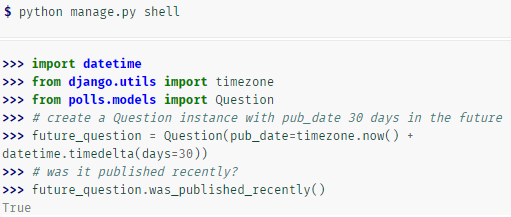
\includegraphics[scale=1]{figuras/3/35/352/img1.png}
%\caption{Agregamos el namespace a \textbf{polls/urls.py}}
\end{center}
\end{figure}

Como las cosas en el futuro no son "recientes", esto es claramente incorrecto.

\subsubsection*{Creamos un Test para exponer al Bug}

Lo que acabamos de hacer en el \textit{shell} para probar el problema es exactamente lo que podemos hacer en una prueba automatizada, así que vamos a convertir eso en una prueba automatizada.

Un lugar convencional para las pruebas de una aplicación es en el archivo \textit{tests.py} de la aplicación; el sistema de prueba encontrará pruebas automáticamente en cualquier archivo cuyo nombre comience con prueba.

Ponga lo siguiente en el archivo \textit{tests.py} en la aplicación de encuestas:

\begin{figure}[H]
\begin{center}
\includegraphics[scale=1]{figuras/3/35/352/img2.png}
%\caption{Agregamos el namespace a \textbf{polls/urls.py}}
\end{center}
\end{figure}

Aquí hemos creado una subclase {\href{https://docs.djangoproject.com/en/3.0/topics/testing/tools/\#django.test.TestCase}{\textcolor{B}{django.test.TestCase}}} con un método que crea una instancia de \textbf{Question} con \textcolor{G}{pub\_date} en el futuro. Luego verificamos el resultado de \textcolor{G}{was\_published\_recently()}, que debería ser falso.

\subsubsection{Corriendo Testeos}
Podemos correr nuestro test desde la terminal:
\begin{figure}[H]
\begin{center}
\includegraphics[scale=1]{figuras/3/35/354/img1.png}
%\caption{Agregamos el namespace a \textbf{polls/urls.py}}
\end{center}
\end{figure}
Y vas a ver algo como:
\begin{figure}[H]
\begin{center}
\includegraphics[scale=0.9]{figuras/3/35/354/img2.png}
%\caption{Agregamos el namespace a \textbf{polls/urls.py}}
\end{center}
\end{figure}

\begin{table}[H]
	\begin{tabular}{||c||}
	\hline \\
	\begin{Large}
		\textbf{¿Tienes un error diferente?}
	\end{Large}
	\\\\		
Si, en cambio, está obteniendo un \textcolor{R}{NameError} aquí, es posible que haya omitido un paso en la\\ \textit{Parte 2} donde agregamos las importaciones de \textit{fecha y hora} y \textit{zona horaria} a \textbf{polls/models.py}.\\ Copie las importaciones de esa sección e intente ejecutar sus pruebas nuevamente.
	\\\\ \hline 	
	\end{tabular}			
\end{table}		

Lo que paso es esto:
\begin{itemize}
\item \textbf{manage.py test polls} busco el archivo \textit{tests.py} en la aplicación \textit{polls}.

\item Este encontró una subclase {\href{https://docs.djangoproject.com/en/3.0/topics/testing/tools/\#django.test.TestCase}{\textcolor{B}{django.test.TestCase}}} 

\item Este crea una base de datos adicional para el propósito del test. 

\item Este busca los metodos de testeos, los cuales son todos los métodos que empiezan con \textbf{test}.

\item 
En \textcolor{G}{test\_was\_published\_recently\_with\_future\_question} se crea una instancia de \textbf{Question} cuyo campo \textit{pub\_date} estará unos 30 días en el futuro respecto del día presente. 

\item 
... y usando el método \textcolor{G}{assertIs()}, este descubre que \textcolor{G}{was\_published\_recently()} devuelve \text{R}{True}, sabiendo que queríamos que este devuelva \text{R}{False}. 
\end{itemize}

La prueba nos informa qué prueba falló e incluso la línea en la que ocurrió la falla.

\subsubsection{Arreglamos el Bug}
Ya sabemos cuál es el problema: \textcolor{G}{Question.was\_published\_recently()} debería devolver \textcolor{R}{False} si su \textcolor{G}{pub\_date} está en el futuro. Modifiquemos el método en \textit{models.py}, para que solo devuelva True si la fecha también está en el pasado:
\begin{figure}[H]
\begin{center}
\includegraphics[scale=1]{figuras/3/35/355/img1.png}
%\caption{Agregamos el namespace a \textbf{polls/urls.py}}
\end{center}
\end{figure}
Corriendo otra vez el comando del testeo, deberíamos ver lo siguiente:
\begin{figure}[H]
\begin{center}
\includegraphics[scale=1]{figuras/3/35/355/img2.png}
%\caption{Agregamos el namespace a \textbf{polls/urls.py}}
\end{center}
\end{figure}
Entonces, lo que hicimos fue identificar un error mediante el test que escribimos, luego corregimos el error que en este caso estaba en la método \textcolor{G}{Question.was\_published\_recently()} dentro del modelo \textbf{Question}, cuando este pasa el test el modelo esta correctamente escrito.

\subsubsection{Tests más completos}
Mientras estamos aquí, podemos precisar el método \textcolor{G}{was\_published\_recently()}; de hecho, sería vergonzoso si al corregir un error hubiéramos introducido otro.

Agregue dos métodos de prueba más a la misma clase, para probar el comportamiento del método de manera más integral:
\begin{figure}[H]
\begin{center}
\includegraphics[scale=1]{figuras/3/35/356/img1.png}
%\caption{Agregamos el namespace a \textbf{polls/urls.py}}
\end{center}
\end{figure}
Y ahora tenemos tres pruebas que confirman que \textcolor{G}{Question.was\_published\_recently()} devuelve valores razonables para preguntas pasadas, recientes y futuras.

Una vez más, las encuestas son una aplicación mínima, pero por compleja que sea en el futuro y cualquier otro código con el que interactúe, ahora tenemos alguna garantía de que el método para el que hemos escrito las pruebas se comportará de la manera esperada.

\subsubsection{Testeando vistas}
La aplicación de encuestas es bastante indiscriminada: publicará cualquier pregunta, incluidas aquellas cuyo campo \textcolor{G}{pub\_date} se encuentre en el futuro. Deberíamos mejorar esto. Establecer una \textcolor{G}{pub\_date} en el futuro debería significar que la Pregunta se publica en ese momento, pero invisible hasta ese momento.

\subsubsection*{\underline{Tests para vistas}}
Cuando solucionamos el error anterior, primero escribimos la prueba y luego el código para solucionarlo. De hecho, ese fue un ejemplo de desarrollo basado en pruebas, pero en realidad no importa en qué orden hagamos el trabajo.

En nuestra primera prueba, nos centramos estrechamente en el comportamiento interno del código. Para esta prueba, queremos verificar su comportamiento, ya que lo experimentaría un usuario a través de un navegador web.

Antes de intentar arreglar cualquier cosa, echemos un vistazo a las herramientas a nuestra disposición.

\subsubsection*{\underline{El cliente de pruebas de \django{}}}
\django{} tiene un cliente de testeo para simular con interactua el usuario con el codigo al nivel de las vistas. Podemos usarlo mediante el \textit{shell} o \textit{tests.py}

Comenzaremos nuevamente con el \textit{shell}, donde debemos hacer un par de cosas que no serán necesarias en \textit{tests.py}. El primero es configurar el entorno de prueba en el \textit{shell}:
\begin{figure}[H]
\begin{center}
\includegraphics[scale=1]{figuras/3/35/357/img1.png}
%\caption{Agregamos el namespace a \textbf{polls/urls.py}}
\end{center}
\end{figure}

{\href{https://docs.djangoproject.com/en/3.0/topics/testing/advanced/\#django.test.utils.setup_test_environment}{\textcolor{B}{setup\_test\_environment()}}}
 instala un renderizador de plantillas que nos permitirá examinar algunos atributos adicionales en las respuestas, como \textcolor{G}{response.context} que de otro modo no estaría disponible. Tenga en cuenta que este método no configura una base de datos de prueba, por lo que lo siguiente se ejecutará en la base de datos existente y el resultado puede diferir ligeramente dependiendo de las preguntas que ya haya creado. Es posible que obtenga resultados inesperados si su  \textcolor{G}{TIME\_ZONE} en \textit{settings.py} no es correcta. Si no recuerda haberlo configurado antes, verifíquelo antes de continuar.

A continuación, necesitamos importar la clase de cliente de prueba (más adelante en \textit{tests.py} usaremos la clase \textcolor{G}{django.test.TestCase}, que viene con su propio cliente, por lo que no será necesario):
\begin{figure}[H]
\begin{center}
\includegraphics[scale=1]{figuras/3/35/357/img2.png}
%\caption{Agregamos el namespace a \textbf{polls/urls.py}}
\end{center}
\end{figure}

Con esto listo, podemos decirle al cliente que haga algunos trabajos para nosotros:

\begin{figure}[H]
\begin{center}
\includegraphics[scale=1]{figuras/3/35/357/img3.png}
%\caption{Agregamos el namespace a \textbf{polls/urls.py}}
\end{center}
\end{figure}

\subsubsection*{\underline{Mejorando nuestra vista}}
La lista de encuestas muestra encuestas que aún no se han publicado (es decir, aquellas que tengan una fecha de publicación en el futuro). Vamos a arreglar eso.

En la parte 4 presentamos una vista basada en clases, basada en \textbf{ListView}:
\begin{figure}[H]
\begin{center}
\includegraphics[scale=1]{figuras/3/35/357/img4.png}
%\caption{Agregamos el namespace a \textbf{polls/urls.py}}
\end{center}
\end{figure}
Debemos corregir el \textcolor{G}{get\_queryset()}
 y cambiarlo para que también verifique la fecha comparándola con \textit{timezone.now()}. Primero necesitamos agregar una importación y luego corregir dicho método:
\begin{figure}[H]
\begin{center}
\includegraphics[scale=1]{figuras/3/35/357/img5.png}
%\caption{Agregamos el namespace a \textbf{polls/urls.py}}
\end{center}
\end{figure}
\textcolor{G}{Question.objects.filter(pub\_date\_\_lte = timezone.now ())} devuelve un conjunto de consultas que contiene preguntas cuyo \textit{pub\_date} es menor o igual a, es decir, anterior o igual a \textcolor{G}{timezone.now}.

\subsubsection*{\underline{Testeamos nuestra vista}}
Ahora podes asegurarte de que esto se comporta como esperas al activar el servidor de ejecución, cargar el sitio en su navegador, crear preguntas con fechas en el pasado y en el futuro, y verificar que solo se enumeren los que se han publicado. Esto es medio embole, así que tambien vamos a crear una prueba basada en nuestra sesión de \textit{shell} anterior.

Agreguemos lo siguiente al \textit{tests.py}:
\begin{figure}[H]
\begin{center}
\includegraphics[scale=0.8]{figuras/3/35/357/img6.png}
%\caption{Agregamos el namespace a \textbf{polls/urls.py}}
\end{center}
\end{figure}

\begin{figure}[H]
\begin{center}
\includegraphics[scale=0.8]{figuras/3/35/357/img7.png}
\includegraphics[scale=0.8]{figuras/3/35/357/img8.png}
%\caption{Agregamos el namespace a \textbf{polls/urls.py}}
\end{center}
\end{figure}

A ver, tratemos de entender esto. 

La primera es una función de acceso directo a preguntas, \textcolor{G}{create\_question}, se usa para tomar algunas repeticiones del proceso de creación de preguntas.

Por otro lado, \textcolor{G}{test\_no\_questions} no crea ninguna pregunta, pero comprueba el mensaje: "No hay encuestas disponibles". y verifica que la última lista de preguntas está vacía. Tenga en cuenta que la clase {\href{https://docs.djangoproject.com/en/3.0/topics/testing/tools/\#django.test.TestCase}{\textcolor{B}{django.test.TestCase}}} proporciona algunos métodos de aserción adicionales. En estos ejemplos, utilizamos {\href{https://docs.djangoproject.com/en/3.0/topics/testing/tools/\#django.test.SimpleTestCase.assertContains}{\textcolor{B}{assertContains()}}} y {\href{https://docs.djangoproject.com/en/3.0/topics/testing/tools/\#django.test.TransactionTestCase.assertQuerysetEqual}{\textcolor{B}{assertQuerysetEqual()}}}.

En \textcolor{G}{test\_past\_question}, creamos una pregunta y verificamos que aparezca en la lista.

En \textcolor{G}{test\_future\_question}, creamos una pregunta con \textcolor{G}{pub\_date} en el futuro. La base de datos se restablece para cada método de prueba, por lo que la primera pregunta ya no está allí, y nuevamente el índice no debería tener ninguna pregunta.

Y así. En efecto, estamos utilizando las pruebas para contar una historia de la entrada del administrador y la experiencia del usuario en el sitio, y verificando que en cada estado y para cada nuevo cambio en el estado del sistema, se publiquen los resultados esperados.

\subsubsection*{\underline{Testeamos el DetilView}}
Lo que tenemos funciona bien; sin embargo, aunque las preguntas futuras no aparezcan en el índice, los usuarios aún pueden comunicarse con ellas si conocen o adivinan la \textbf{URL} correcta. Por lo tanto, debemos agregar una restricción similar a \textbf{DetailView}:
\begin{figure}[H]
\begin{center}
\includegraphics[scale=1]{figuras/3/35/357/img9.png}
%\caption{Agregamos el namespace a \textbf{polls/urls.py}}
\end{center}
\end{figure}
Agregaremos algunas pruebas, para verificar que una Pregunta cuya \textcolor{G}{pub\_date} esté en el pasado se pueda mostrar, y que una con \textcolor{G}{pub\_date} en el futuro no:

\begin{figure}[H]
\begin{center}
\includegraphics[scale=1]{figuras/3/35/357/img10.png}
%\caption{Agregamos el namespace a \textbf{polls/urls.py}}
\end{center}
\end{figure}

\subsubsection{Algunas ideas para la creacion de otros tests}
Deberíamos agregar un método \textcolor{G}{get\_queryset} similar a \textcolor{G}{ResultsView} y crear una nueva clase de prueba para esa vista. Será muy similar a lo que acabamos de crear; de hecho habrá mucha repetición.

También podríamos mejorar nuestra aplicación de otras maneras, agregando pruebas en el camino. Por ejemplo, es una tontería que las preguntas se puedan publicar en el sitio que no tiene opciones. Por lo tanto, nuestras opiniones podrían verificar esto y excluir tales Preguntas. Nuestras pruebas crearían una pregunta sin opciones y luego comprobarían que no está publicada, así como crearían una pregunta similar con opciones y comprobarían que está publicada.

Tal vez a los usuarios administradores registrados se les debería permitir ver preguntas no publicadas, pero no visitantes comunes. Una vez más: lo que sea necesario agregar al software para lograr esto debe ir acompañado de una prueba, ya sea que escriba la prueba primero y luego haga que el código pase la prueba, o calcule primero la lógica en su código y luego escriba una prueba.

En cierto momento, seguramente verás tus pruebas y te preguntarás si tu código sufre de hinchazón de prueba, lo que nos lleva a:

\subsubsection*{\underline{Cuando hacemos pruebas, más es mejor}}
Puede parecer que nuestras pruebas están fuera de control. A este ritmo, pronto habrá más código en nuestras pruebas que en nuestra aplicación, y la repetición no es estética, en comparación con la elegante concisión del resto de nuestro código.

No importa. Déjalos crecer. En su mayor parte, puede escribir una prueba una vez y luego olvidarse de ella. Continuará realizando su útil función a medida que continúe desarrollando su programa.

Algunas veces las pruebas deberán actualizarse. Supongamos que modificamos nuestras opiniones para que solo se publiquen Preguntas con opciones. En ese caso, muchas de nuestras pruebas existentes fallarán, diciéndonos exactamente qué pruebas deben modificarse para actualizarlas, por lo que las pruebas ayudan a cuidarse a sí mismas.

En el peor de los casos, a medida que continúe desarrollando, es posible que tenga algunas pruebas que ahora son redundantes. Incluso eso no es un problema; en la prueba de redundancia es algo bueno.

Mientras sus exámenes estén organizados de manera sensata, no serán inmanejables. Las buenas reglas generales incluyen tener:
\begin{itemize}
\item 
un TestClass separado para cada modelo o vista

\item un método de prueba separado para cada conjunto de condiciones que desea probar


\item nombres de métodos de prueba que describen su función 
\end{itemize}

\subsubsection*{\underline{Pruebas adicionales}}
Este tutorial solo presenta algunos de los conceptos básicos de las pruebas. Hay mucho más que puede hacer y una serie de herramientas muy útiles a su disposición para lograr algunas cosas muy inteligentes.

Por ejemplo, si bien nuestras pruebas aquí han cubierto parte de la lógica interna de un modelo y la forma en que nuestras vistas publican información, puede usar un marco "en el navegador" como {\href{http://seleniumhq.org}{\textcolor{B}{Selenium}}}
 para probar la forma en que su \textbf{HTML} se procesa en un navegador. Estas herramientas le permiten verificar no solo el comportamiento de su código \django{}, sino también, por ejemplo, de su \textbf{JavaScript}. ¡Es bastante ver que las pruebas inician un navegador y comienzan a interactuar con su sitio, como si un ser humano lo condujera! \django{} incluye {\href{https://docs.djangoproject.com/en/3.0/topics/testing/tools/\#django.test.LiveServerTestCase}{\textcolor{B}{LiveServerTestCase}}}
 para facilitar la integración con herramientas como {\href{http://seleniumhq.org}{\textcolor{B}{Selenium}}}.

Si tiene una aplicación compleja, es posible que desee ejecutar pruebas automáticamente con cada confirmación con el fin de una {\href{https://en.wikipedia.org/wiki/Continuous\_integration}{\textcolor{B}{integración continua}}}, de modo que el control de calidad sea en sí mismo, al menos parcialmente, automatizado.

Una buena manera de detectar partes no probadas de su aplicación es verificar la cobertura del código. Esto también ayuda a identificar el código frágil o incluso muerto. Si no puede probar un fragmento de código, generalmente significa que el código debe ser refactorizado o eliminado. La cobertura ayudará a identificar el código muerto. Vea {\href{https://docs.djangoproject.com/en/3.0/topics/testing/advanced/\#topics-testing-code-coverage}{\textcolor{B}{Integración con \textit{coverage.py}}}} para más detalles.

Las pruebas en \django{} ({\href{https://docs.djangoproject.com/en/3.0/topics/testing/}{\textcolor{B}{Testing in Django}}}) tienen información completa sobre las pruebas.


\newpage
\subsection{Escribiendo tu primera aplicación \django{}, parte 6}
 Ya hemos creado el proyecto, la aplicacion de encuesta y todo el back de la pagina y ahora agregaremos una hoja de estilo y una imagen, para tener un poco más de front.

Además del \textbf{HTML} generado por el servidor, las aplicaciones web generalmente necesitan servir archivos adicionales, como imágenes, \textbf{JavaScript} o \textbf{CSS}, necesarios para representar la página web completa. En \django{}, nos referimos a estos archivos como "archivos estáticos".

Para proyectos pequeños, esto no es un gran problema, ya que puede mantener los archivos estáticos en algún lugar donde su servidor web pueda encontrarlos. Sin embargo, en proyectos más grandes, especialmente aquellos compuestos por múltiples aplicaciones, tratar con los múltiples conjuntos de archivos estáticos proporcionados por cada aplicación comienza a ser complicado.

Para eso es \textcolor{G}{django.contrib.staticfiles}: recopila archivos estáticos de cada una de sus aplicaciones (y de cualquier otro lugar que especifique) en una única ubicación que se pueda servir fácilmente en producción.

\subsubsection{Personaliza el aspecto de tu aplicación}
Primero, cree un directorio llamado static en su directorio de encuestas. Django buscará archivos estáticos allí, de manera similar a cómo Django encuentra plantillas dentro de encuestas / templates /.

La configuración {\href{https://docs.djangoproject.com/en/3.0/ref/settings/\#std:setting-STATICFILES\_FINDERS}{\textcolor{G}{STATICFILES\_FINDERS}}} de \django{} contiene una lista de buscadores que saben cómo descubrir archivos estáticos de varias fuentes. Uno de los valores predeterminados es \textcolor{G}{AppDirectoriesFinder}, que busca un subdirectorio "estático" en cada una de las \textcolor{G}{INSTALLED\_APPS}, como el de las encuestas que acabamos de crear. El sitio de administración utiliza la misma estructura de directorio para sus archivos estáticos.

Dentro del directorio estático que acaba de crear, cree otro directorio llamado encuestas y dentro de ese, cree un archivo llamado \textit{style.css}. En otras palabras, su hoja de estilo debe estar en \textbf{polls/static/polls/style.css}. Debido a cómo funciona el buscador de archivos estáticos \textcolor{G}{AppDirectoriesFinder}, puede referirse a este archivo estático en \django{} como \textbf{polls/style.css}, similar a cómo hace referencia a la ruta de las plantillas.
\begin{table}[H]
	\begin{tabular}{||c||}
	\hline \\
	\begin{Large}
	\textbf{static file namespacing}
	\end{Large}
	\\\\		
Al igual que las plantillas, podríamos evitar poner nuestros archivos estáticos directamente en \textbf{polls/static}\\ (en lugar de crear otro subdirectorio de encuestas), pero en realidad sería una mala idea.\\ \django{} elegirá el primer archivo estático que encuentre cuyo nombre coincida,\\ y si tuviera un archivo estático con el mismo nombre en una aplicación\\ diferente, \django no podría distinguirlos.\\ Necesitamos poder apuntar a Django al correcto, y la mejor manera\\ de asegurar esto es espaciando los nombres.\\ Es decir, al poner esos archivos estáticos \\dentro de otro directorio nombrado para la aplicación misma.
	\\\\ \hline 	
	\end{tabular}			
\end{table}		

Ponga el siguiente código en esa hoja de estilo (\textbf{polls/static/ polls/style.css}):
\begin{figure}[H]
\begin{center}
\includegraphics[scale=0.8]{figuras/3/36/361/img1.png}
%\caption{Agregamos el namespace a \textbf{polls/urls.py}}
\end{center}
\end{figure}
Luego, agregamos lo siguiente a \textbf{polls/templates/polls/index.html}:
\begin{figure}[H]
\begin{center}
\includegraphics[scale=0.8]{figuras/3/36/361/img2.png}
%\caption{Agregamos el namespace a \textbf{polls/urls.py}}
\end{center}
\end{figure}

La etiqueta de plantilla \textcolor{R}{\{\% static \%\}} genera la \textbf{URL} absoluta de los archivos estáticos.

Eso es todo lo que necesitas hacer para el desarrollo.

Inicie el servidor (o reinícielo)

\subsubsection{Imagen de fondo}
A continuación, crearemos un subdirectorio para imágenes. Cree un subdirectorio de imágenes en el directorio encuestas \textbf{/static/polls/}. Dentro de este directorio, coloque una imagen llamada background.gif. En otras palabras, coloque su imagen en encuestas \textbf{/static/polls/images/background.gif}.

Luego, agregue a su hoja de estilo (\textbf{polls/static/polls/style.css}):
\begin{figure}[H]
\begin{center}
\includegraphics[scale=1]{figuras/3/36/361/img1.png}
%\caption{Agregamos el namespace a \textbf{polls/urls.py}}
\end{center}
\end{figure}
Luego, reinicia el navegador.
\begin{table}[H]
	\begin{tabular}{||c||}
	\hline \\
	\begin{Large}
	\textbf{Cuidado!}
	\end{Large}
	\\\\		
	
Por supuesto, la etiqueta de plantilla \textcolor{R}{\{\% static \%\}} no está disponible\\ para su uso en archivos estáticos como su hoja de estilo que no son generados por \django{}.\\ Siempre debe usar rutas relativas para vincular sus archivos estáticos entre sí,\\ porque luego puede cambiar {\href{https://docs.djangoproject.com/en/3.0/ref/settings/\#std:setting-STATIC\_URL}{\textcolor{B}{STATIC\_URL}}}
 (utilizado por la etiqueta de plantilla {\href{https://docs.djangoproject.com/en/3.0/ref/templates/builtins/\#std:templatetag-static}{\textcolor{B}{estática}}} para generar sus URL)\\ sin tener que modificar también un montón de rutas en sus archivos estáticos.
	\\\\ \hline 	
	\end{tabular}			
\end{table}		


Estos son los conceptos básicos. Para obtener más detalles sobre la configuración y otros bits incluidos en el marco, consulte {\href{https://docs.djangoproject.com/en/3.0/howto/static-files/}{\textcolor{B}{los procedimientos de archivos estáticos}}} y {\href{https://docs.djangoproject.com/en/3.0/ref/contrib/staticfiles/}{\textcolor{B}{la referencia de archivos estáticos}}}. La {\href{https://docs.djangoproject.com/en/3.0/howto/static-files/deployment/}{\textcolor{B}{implementación de archivos estáticos}}} explica cómo usar archivos estáticos en un servicio real.








%\begin{figure}[H]
%\begin{center}
%\includegraphics[scale=1]{figuras/3/34/341/img5.png}
%\caption{Agregamos el namespace a \textbf{polls/urls.py}}
%\end{center}
%\end{figure}

%\begin{table}[H]
%	\begin{tabular}{||c||}
%	\hline \\
%	\begin{Large}
%	\textbf{TITULO}
%	\end{Large}
%	\\\\		

%	\\\\ \hline 	
%	\end{tabular}			
%\end{table}		

%{\href{}{\textcolor{B}{}}}
%%%%%%%%%%%%%%%%%%%%%%%%%%%%%%%%%%%%%%%%%%%%%%%%%%%%%%%%%%
%%%%%%%%%%%%%%%%%%%%%%%%%%%%%%%%%%%%%%%%%%%%%%%%%%%%%%%%%%
%%%%%%%%%%%%%%%%%%%%%%%%%%%%%%%%%%%%%%%%%%%%%%%%%%%%%%%%%%
%%%%%%%%%%%%%%%%%%%%%%%%%%%%%%%%%%%%%%%%%%%%%%%%%%%%%%%%%%
\newpage
\section{Referencias}
\subsection{Refes de las partes de los tutoriales}
\begin{itemize}
\item {\textcolor{B}{\href{https://docs.djangoproject.com/en/3.0/intro/tutorial01/}{Parte 1}}}

\item {\textcolor{B}{\href{https://docs.djangoproject.com/en/3.0/intro/tutorial02/}{Parte 2}}}

\item {\href{https://docs.djangoproject.com/en/3.0/intro/tutorial03/}{\textcolor{B}{parte 3}}}

\item {\href{https://docs.djangoproject.com/en/3.0/intro/tutorial04/}{\textcolor{B}{parte 4}}}

\item {\href{https://docs.djangoproject.com/en/3.0/intro/tutorial05/}{\textcolor{B}{parte 5}}}

\item {\href{https://docs.djangoproject.com/en/3.0/intro/tutorial06/}{\textcolor{B}{parte 6}}}

\item {\href{https://docs.djangoproject.com/en/3.0/intro/tutorial07/}{\textcolor{B}{parte 7}}}

\item {\href{https://docs.djangoproject.com/en/3.0/intro/reusable-apps/}{\textcolor{B}{Reusable Apps}}}
\end{itemize}

\subsection{Refes W3School}
\begin{itemize}
\item {\textcolor{B}{\href{https://www.w3schools.com/html/}{Html}}}

\item {\textcolor{B}{\href{https://www.w3schools.com/css/default.asp}{css}}}

\item {\textcolor{B}{\href{https://www.w3schools.com/js/default.asp}{javascript}}}

\item {\textcolor{B}{\href{https://www.w3schools.com/python/default.asp}{Python}}}

\item {\textcolor{B}{\href{https://www.w3schools.com/bootstrap/bootstrap_ver.asp}{Bootstrap}}}
\end{itemize}

\subsection{Atajos}

\begin{itemize}
\item {\textcolor{B}{\href{https://conda.io/projects/conda/en/latest/user-guide/tasks/manage-environments.html\#creating-an-environment-with-commands}{Crear entorno de python con conda}}}


\item {\textcolor{B}{\href{https://unipython.com/cambiar-tu-version-de-python-con-anaconda/}{Cambiar de version de python con conda}}}


\item {\textcolor{B}{\href{http://www.i18nguy.com/unicode/language-identifiers.html}{LANGUAGE\_CODE}}}

\item {\textcolor{B}{\href{https://en.wikipedia.org/wiki/List_of_tz_database_time_zones}{TIME\_ZONE}}}


\end{itemize}


\end{document}